\documentclass[]{article}
\usepackage{caption,subcaption,graphicx,float,url,amsmath,amssymb,tocloft}
\usepackage[hidelinks]{hyperref}
\usepackage[toc,acronym,nonumberlist]{glossaries}
\setacronymstyle{long-short}
\usepackage{glossaries-extra}
\graphicspath{{figs/}} 
\DeclareUnicodeCharacter{2192}{~}
\setlength{\cftsubsecindent}{0em}
\setlength{\cftsecnumwidth}{3em}
\setlength{\cftsubsecnumwidth}{3em}

%opening
\title{
	Notes from Origins of Life\\
	Week 2: Chemical Origins
}

\author{Simon Crase (compiler)\\simon@greenweaves.nz}

\makeglossaries

\loadglsentries{glossary-entries}

\renewcommand{\thesection}{2.\arabic{section}}
\renewcommand{\glstextformat}[1]{\textbf{\em #1}}

\begin{document}

\maketitle

\begin{abstract}
   These are my notes from the $2^{nd}$ week of the Santa Fe Institute Origins of Life Course\cite{sfi2020}. The course aims to push the field of Origins of Life research forward by bringing new and synthetic thinking to the question of how life emerged from an abiotic world.\\
   The content and images contained herein are the intellectual property of the Santa Fe Institute, with the exception of any errors in transcription, which are my own.
   These notes are distributed in the hope that they will be useful,
   but without any warranty, and without even the implied warranty of
   merchantability or fitness for a particular purpose. All feedback is welcome,
   but I don't necessarily undertake to do anything with it.

\end{abstract}

\setcounter{tocdepth}{2}
\tableofcontents
\listoffigures

\section[Introduction]{Introduction--Chris Kempes}

We will take a closer look at the detailed chemistry thought to be important to the origin of life. We will discuss
\begin{itemize}
	\item likely chemistry of the early Earth,
	\item chemistry that may be  fundamental to the origin of life,
	\item what chemistry we know is essential for biochemistry of modern life,
	\item processes that can occur in chemical dynamics, 
	\item types of extreme life that occurs today in a variety of environments.
\end{itemize}


\section{What Did Early Earth Look Like?}

\subsection[Geochemical Landscape]{Geochemical Landscape--Sarah Mauer}

We are going to look at what earth looked like between 4.2 and 3.8 billion years ago, and how that might relate to the origins of life. The first thing to know is what the Geochemical landscape looked like--Figure \ref{fig:GeochemicalLandscape}.

  \begin{itemize}
	\item  Definitely an ocean that was warmer than today's oceans, probably saltier.\footnote{''While this is not my exact field of study, I am told that water-rock-atmosphere equilibriums operate at orders of magnitude faster time scales than planetary evolution. So the ocean “quickly” came to equilibrium with early oceans (maybe a million years or less), then as new rock was exposed, and the atmosphere changed, the equilibrium shifted. The composition may have been different, with more reduced metals for example, but sodium chloride is the most abundant ionic compound and likely always has been.''--Sarah Maurer}\cite{knauth1998salinity} 
	\item Landmasses from volcanic activity, and, maybe, plate tectonics.
	\item On continents, lakes and ponds from precipitation.  Maybe temporary streams from precipitation.
	\item Surfaces composed of minerals, which were good for catalysis and energy production. Today covered with life.
\end{itemize}

\begin{figure}[H]
	\caption[Geochemical Landscape]{Geochemical Landscape after \cite{kitadai2018origins}} \label{fig:GeochemicalLandscape}
	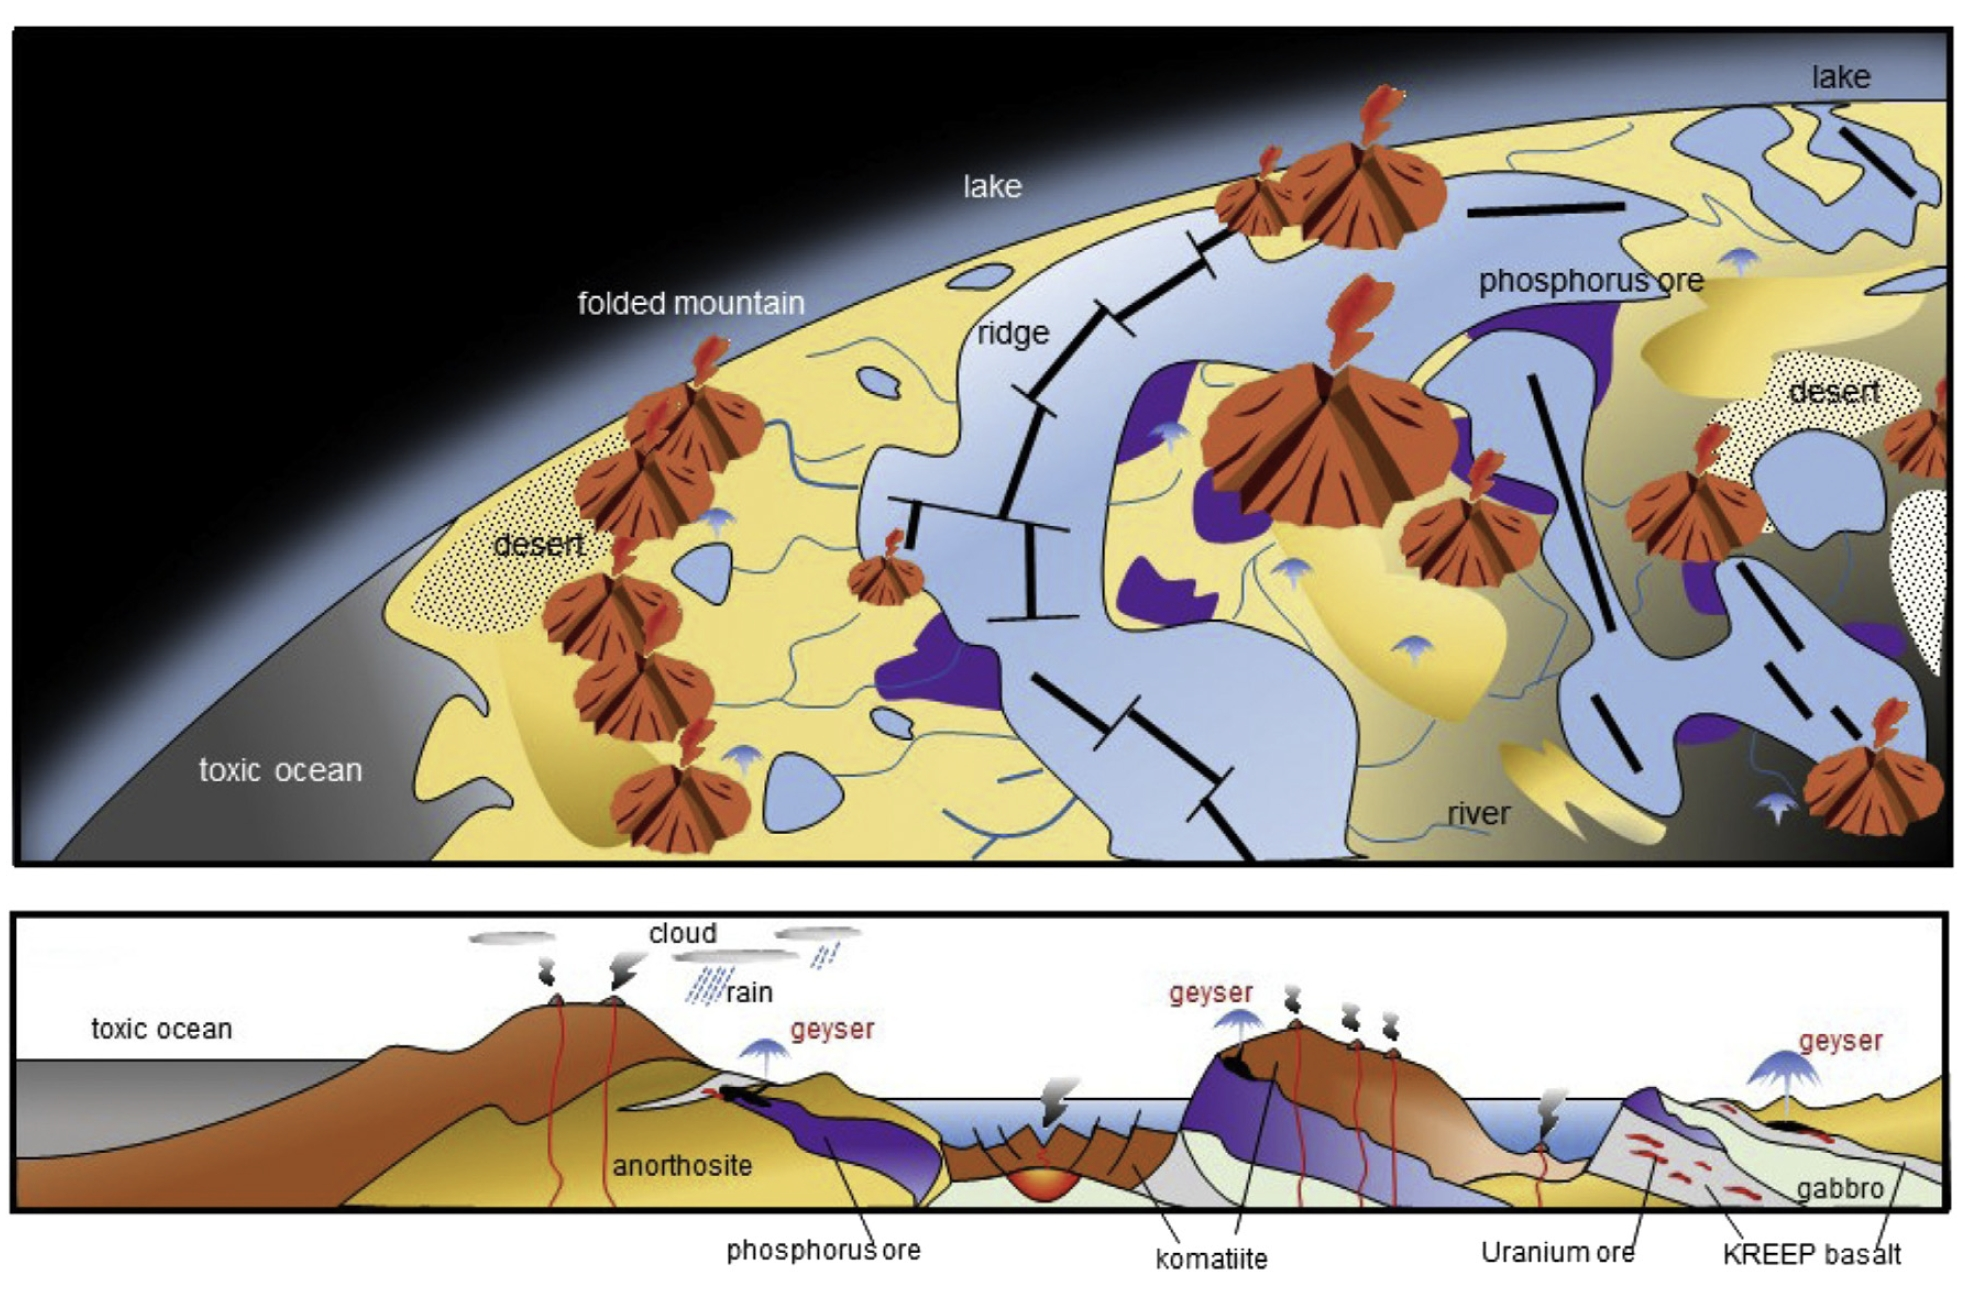
\includegraphics[width=0.9\textwidth]{GeochemicalLandscape}
\end{figure}


\subsubsection{Mixing processes between chemical reactors}

The different chemical reactions that were occurring on early Earth would have been mixed through a variety of different processes, similar to today, so there were likely tides, mixing between the ocean and the inland lakes through evaporation, aerosols, volcanic plumes, carrying molecules to location where different chemistry could occur. All this mixing would lead to a unique chemical library through a variety of different reactions--Figure \ref{fig:MixingProcesses}.
 
\begin{figure}[H]
	\caption[Mixing processes between chemical reactors]{Mixing processes between chemical reactors \cite{stueken2013did}}\label{fig:MixingProcesses}
	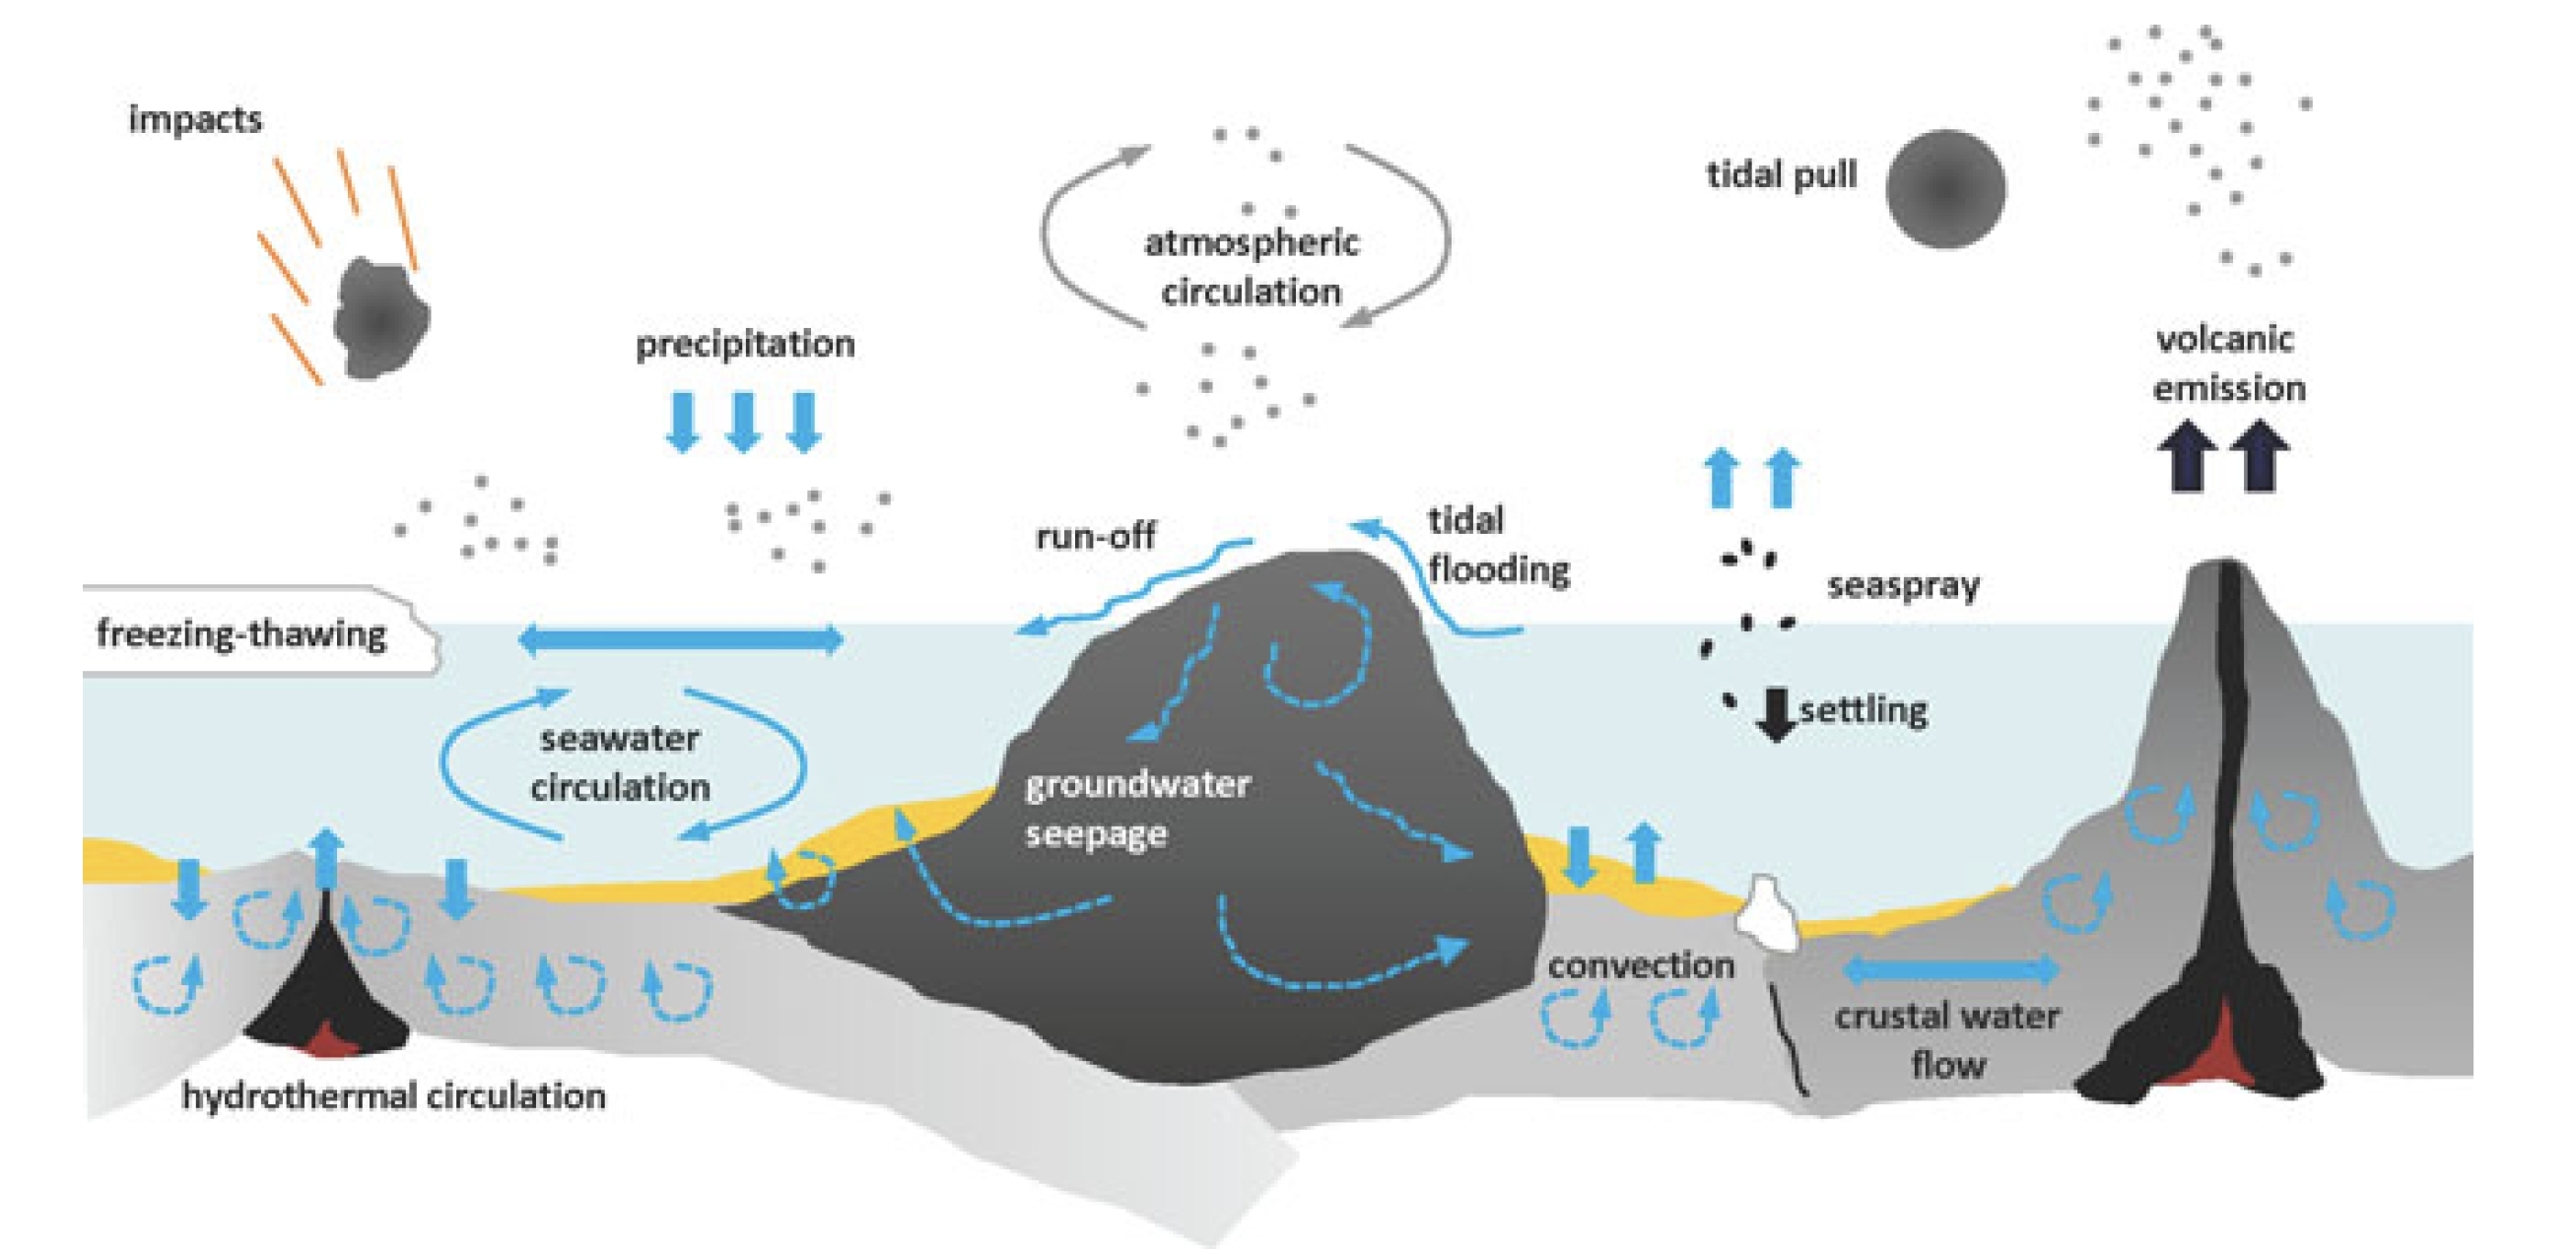
\includegraphics[width=0.8\textwidth]{MixingProcesses}
\end{figure}

  
  
\subsubsection{Geothermal systems}
\begin{figure}[H]
	\caption[Geothermal systems]{Geothermal systems \cite{damer2016field}}
	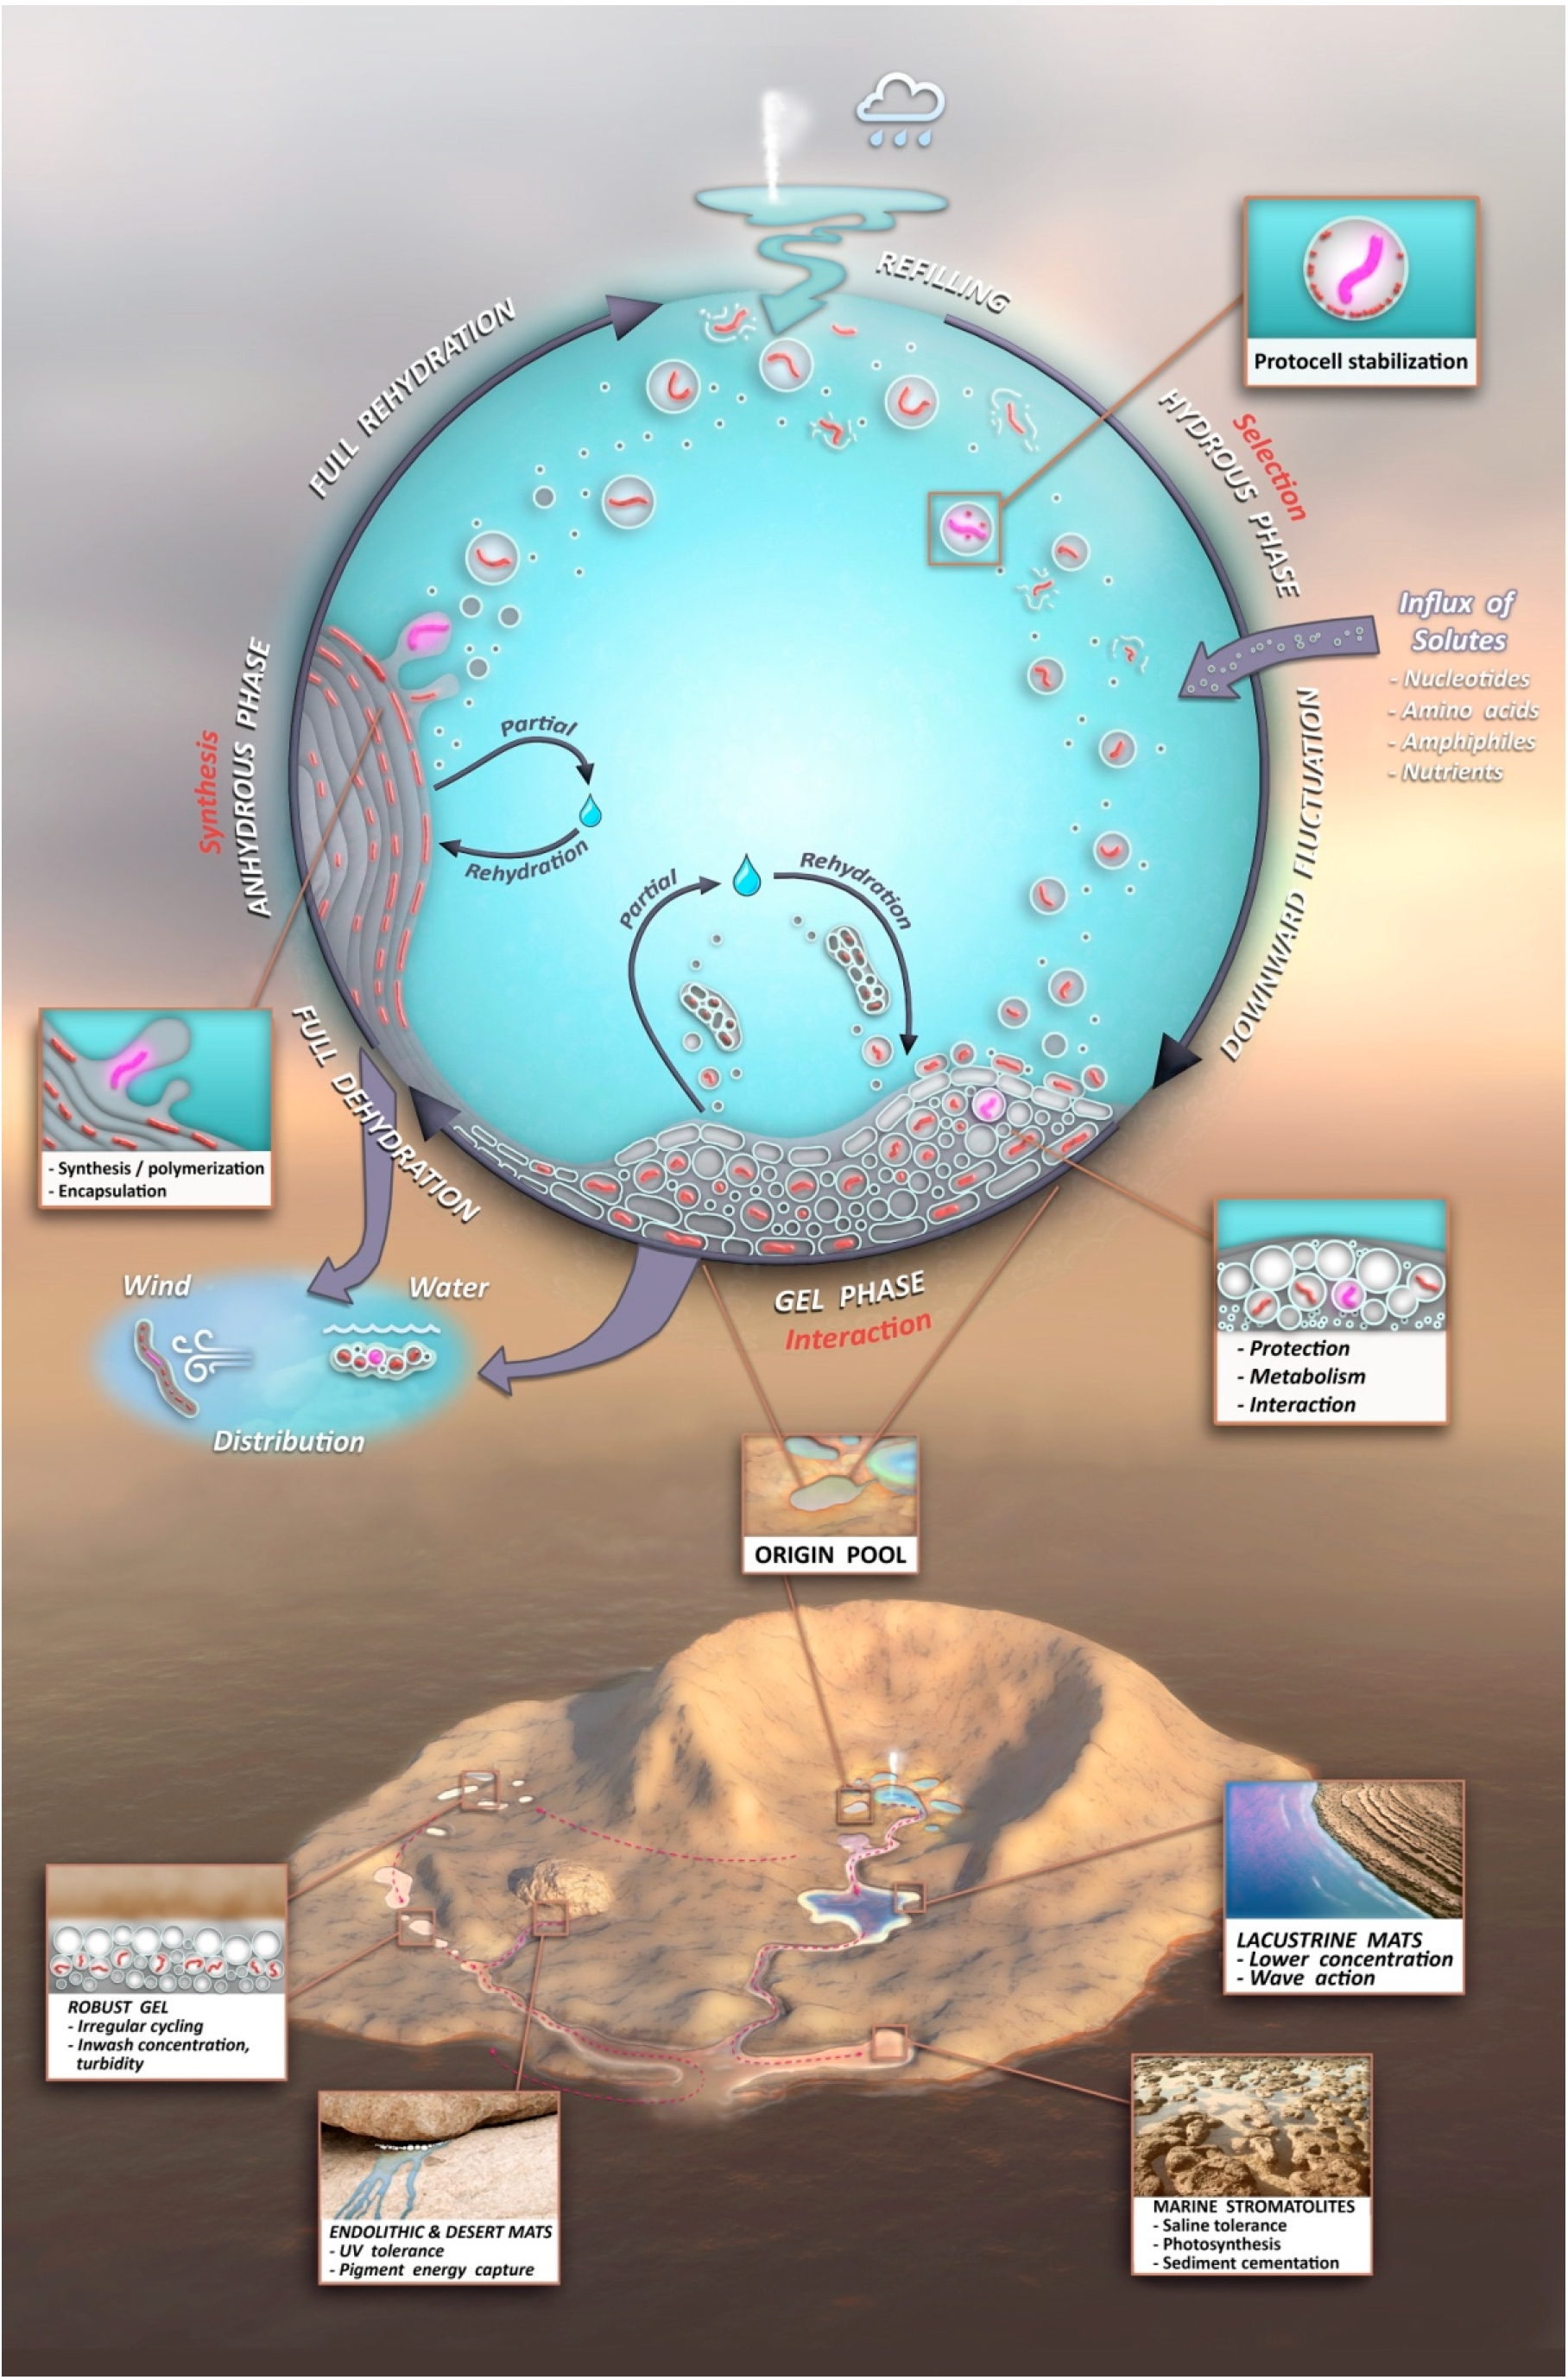
\includegraphics[width=0.9\textwidth]{GeothermalSystems}
\end{figure}

\begin{itemize}
	\item Provide high temperature, high pressure, reduced	reaction products
	\item Fresh water from 	precipitation
	\item Diversity of mineral	surfaces for ”nutrients” and catalysis
\end{itemize}

\subsubsection{Energy Sources}

See \cite{kitadai2018origins}, \cite{stueken2013did}, \cite{damer2016field}, \cite{miller1959organic}, \cite{ehrenfreund2002astrophysical},\cite{dalai2016incubating}, and \cite{chyba1997comets}.

\begin{itemize}
	\item Chemical Energy
	\begin{itemize}
		\item Reducing gases
		\item Radiation
		\item Minerals
	\end{itemize}
	\item Other Energy Sources
	\begin{itemize}
		\item Volcanic lightning
		\item UV-light
		\item High temperature
		\item Pressure
		\item Impacts
	\end{itemize}
\end{itemize}
Figure \ref{fig:MillerUrey} depicts the Miller Urey experiment. It now seems likely that there was no methane in the atmosphere of the early Earth, but but we could use CO2 to derive a different mixture.

\begin{figure}[H]
	\caption[Miller Urey Experiment]{Miller Urey Experiment\cite{miller1959organic}}\label{fig:MillerUrey}
	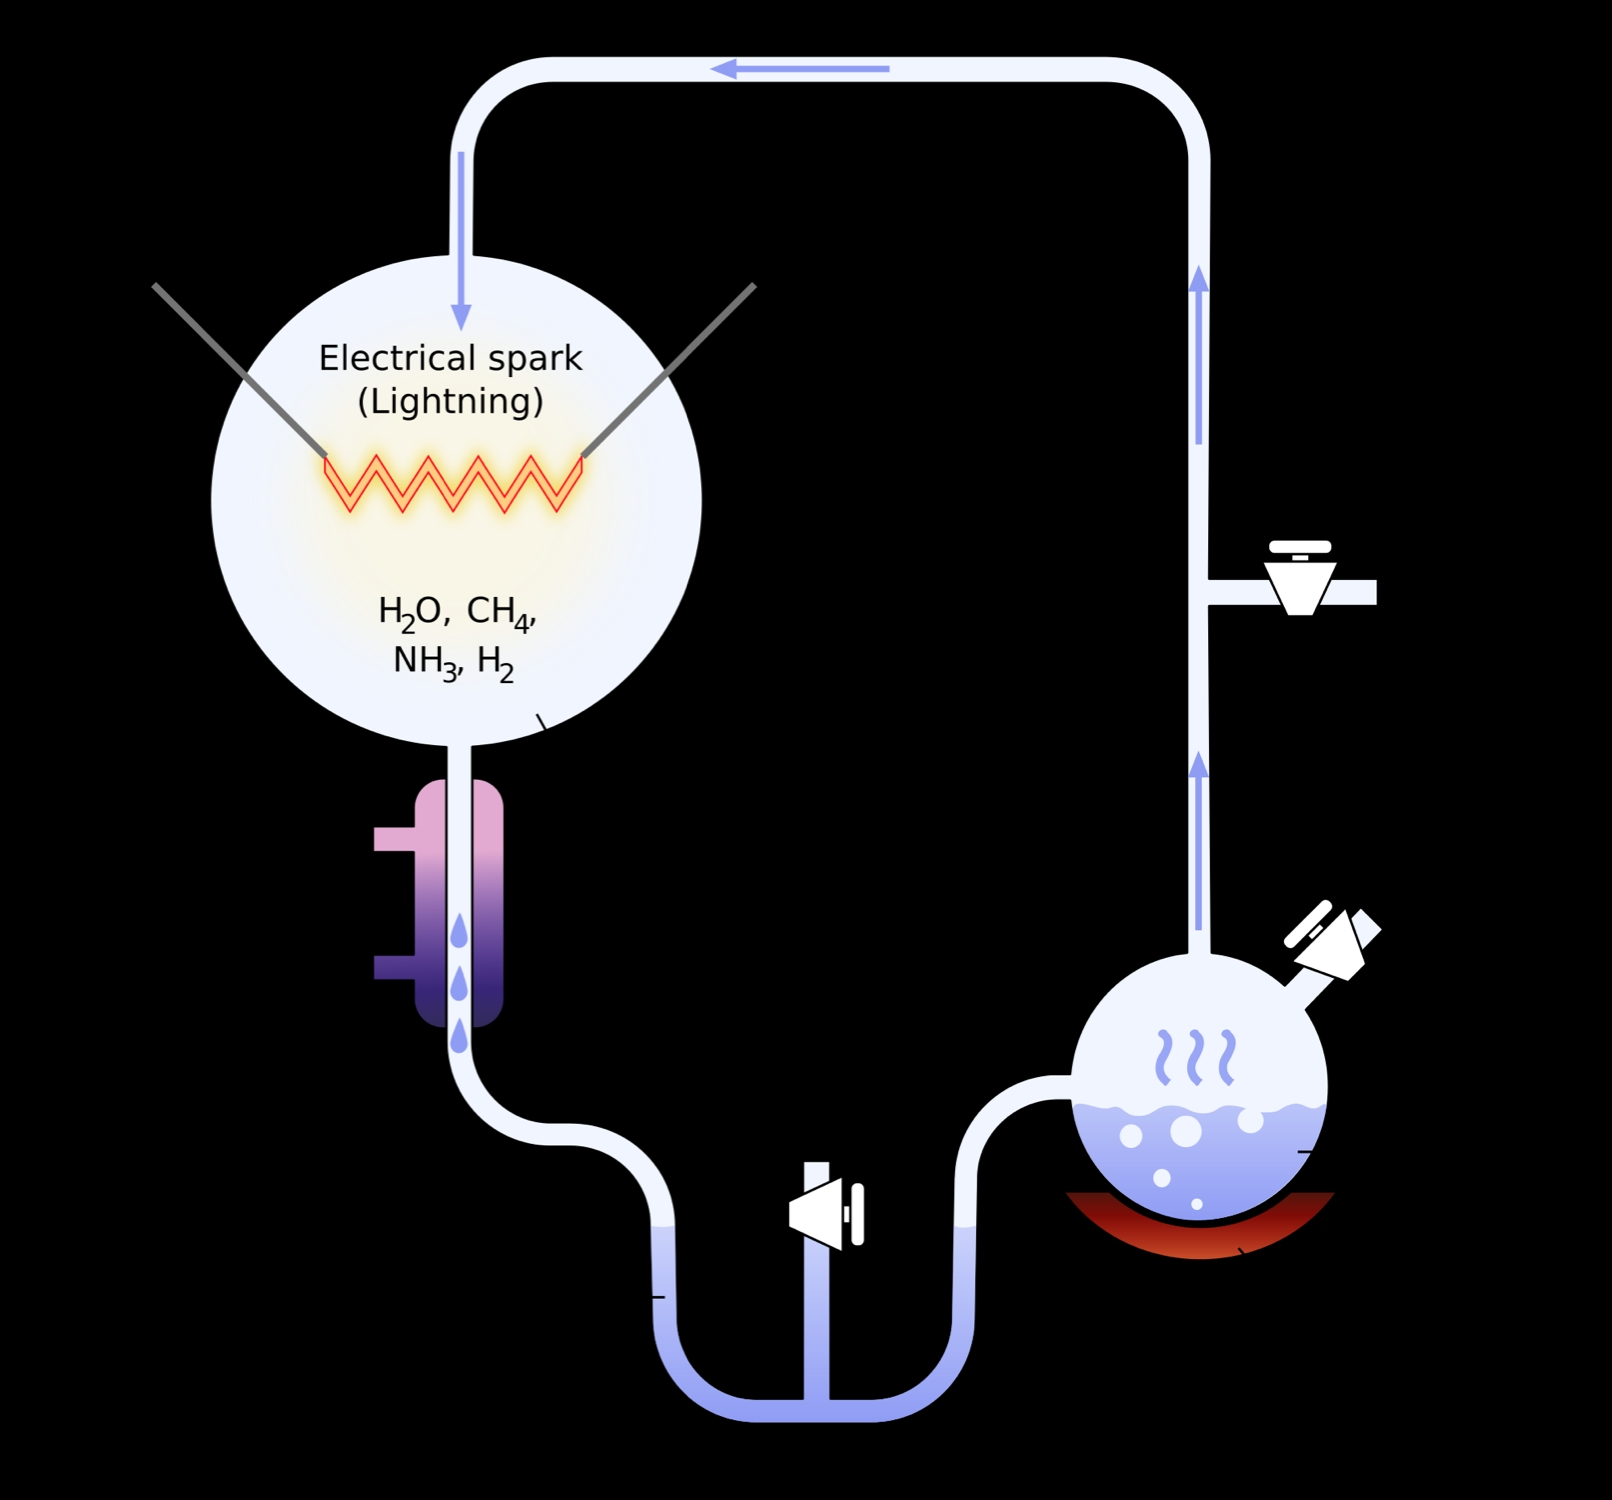
\includegraphics[width=0.45\textwidth]{MillerUrey1}
	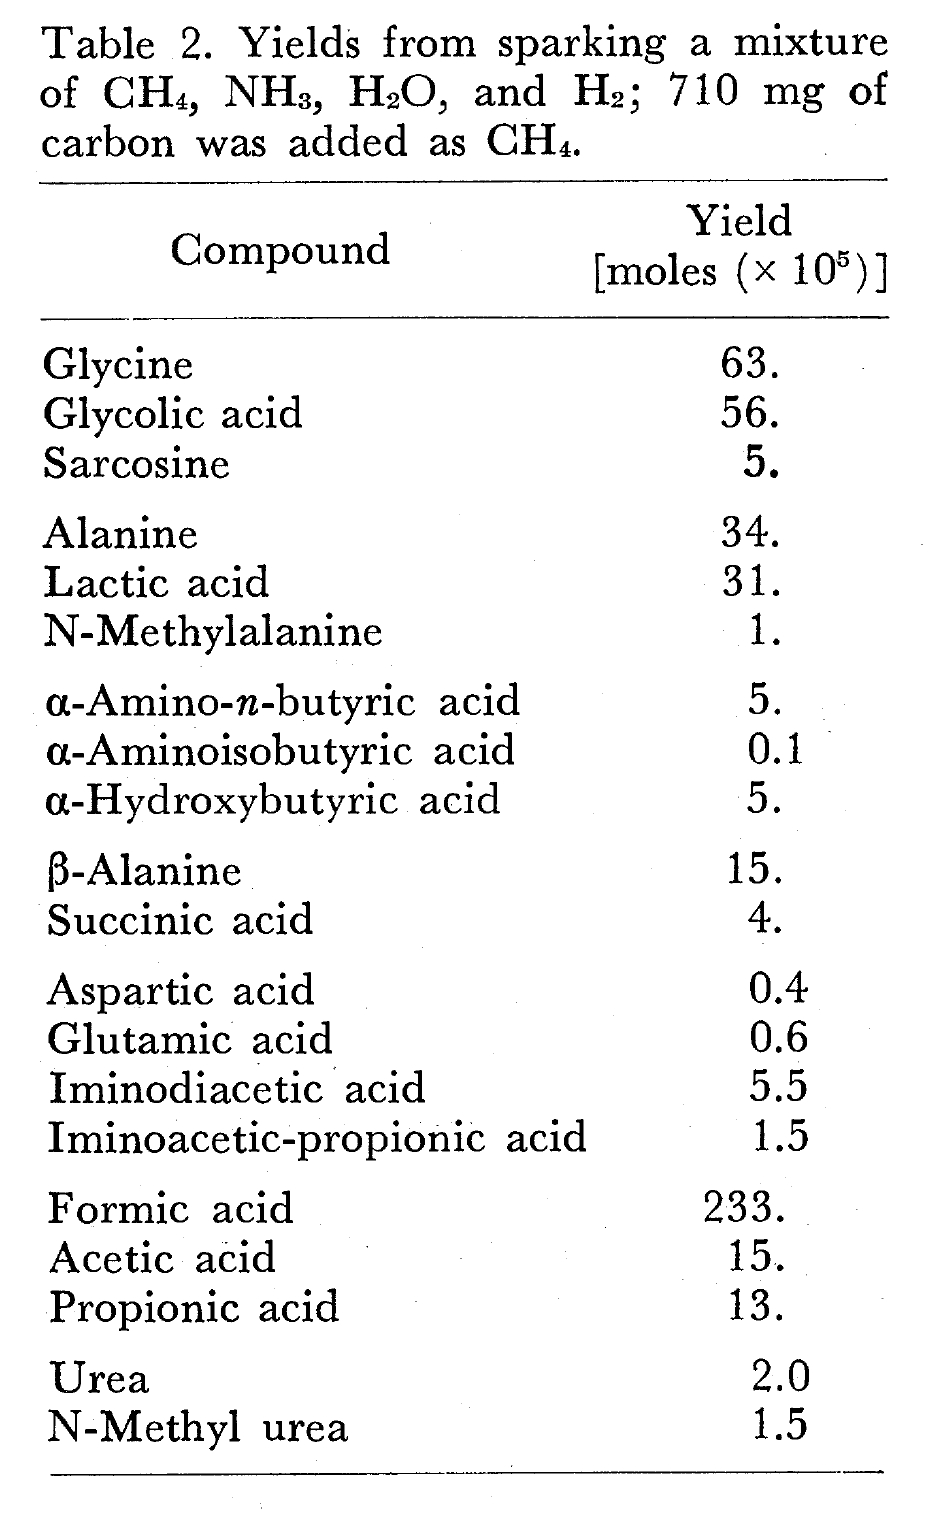
\includegraphics[width=0.45\textwidth]{MillerUrey2}
\end{figure}

The other major source of organic compounds is through interplanetary dust particles--delivery of carbon to Earth from the solar system. When earth was formed the Solar System was still accreting, and smaller particles would have been pulled in by Earth's gravity.  These particles would have had a different chemistry. One of the most famous is the Murchison meteorite--Figure \ref{fig:CarbonaceousChondrites}. It has an interesting library of compounds, including amphiphiles, which could form membrane structures, polycyclic hydrocarbons, alcohols, and some aliphatic hydrocarbons that have could have been metabolic components. When looking at other carbonaceous chondrites  we see that each meteorite has a different library.
\begin{figure}[H]
	\caption[Carbonaceous Chondrites]{Carbonaceous Chondrites after \cite{ehrenfreund2002astrophysical}}\label{fig:CarbonaceousChondrites}
	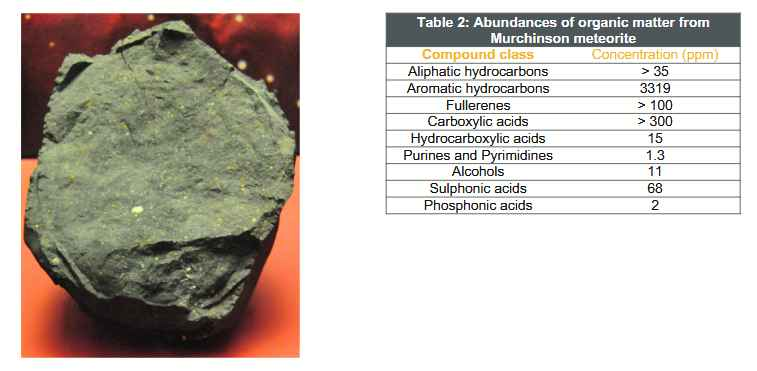
\includegraphics[width=0.8\textwidth]{CarbonaceousChondrites}
\end{figure}


The libraries are produced because the reactions are dependent on the types of energy that hit that particle--Figure \ref{fig:ReactionsInSpace}.

\begin{figure}[H]
	\caption[Reactions In Space]{Reactions In Space after \cite{dalai2016incubating}. UV radiation causes free radicals, which can lead to some strange chemistry.}\label{fig:ReactionsInSpace}
	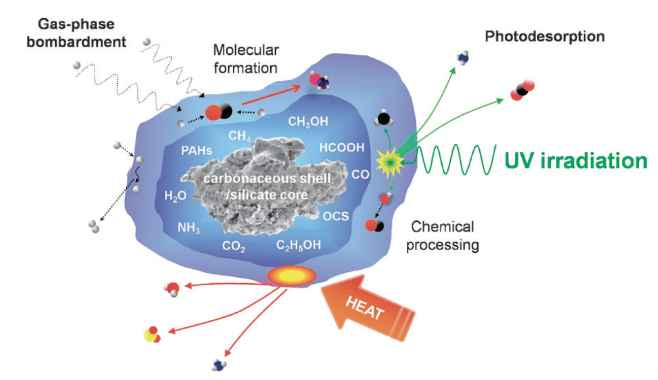
\includegraphics[width=\textwidth]{ReactionsInSpace}
\end{figure}

Was there enough of these reactions to generate a complex chemical that could have led to life? When we estimate how many of all the different events occurred and compile toe different sources of carbon, we estimate about 100 billion kg of prebiotic organic material was delivered to Earth or synthesized on Earth per annum--Figure \ref{fig:SourcesPrebioticOrganicMaterial}. So we think there was enough material to jump-start life.

\begin{figure}[H]
	\begin{center}
		\caption[Sources of Prebiotic of Organic Material]{Sources of Prebiotic of Organic Material after \cite{chyba1997comets}} \label{fig:SourcesPrebioticOrganicMaterial}
		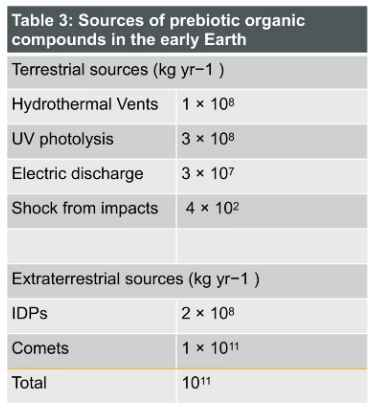
\includegraphics[width=0.8\textwidth]{SourcesPrebioticOrganicMaterial}
	\end{center}
\end{figure}


\subsection[Early Earth Bombardment History]{Early Earth Bombardment History--Nicolle Zellner }

New Views of the Bombardment of the Earth-Moon System, and their effect on our interpretation of the origin of life.

\subsubsection{Why study the Moon?}
\begin{itemize}
	\item Samples and surface are (mostly) undisturbed: no water, no plate-tectonics, no atmosphere.
	\item Samples can be dated ($^{40}Ar/^{39}Ar$, $^{87}Rb/^{87}Sr$, Uranium/Lead etc.)
	\item Craters can be counted, and we can look at superposition of ejecta to estimate age.
\end{itemize}
Lunar cratering rate anchors the impact chronology for the entire (inner) Solar System. We can scale impact fluxes and apply to the other planets.

Figure \ref{fig:LunarImpactFluxModels} shows a number of scenarios.
\begin{figure}[H]
	\caption[Lunar Impact Flux Models]{Lunar Impact Flux Models\cite{zellner2002geochemistry,hartmann1965terrestrial,hartmann1970lunar,hartmann2000time,tera1974isotopic,gomes2005origin}}\label{fig:LunarImpactFluxModels}
	\begin{subfigure}[t]{0.45\textwidth}
		\caption{As we understand solar system formation, there should be a lot of material falling in early, but it starts to decline in intensity going forward.}
		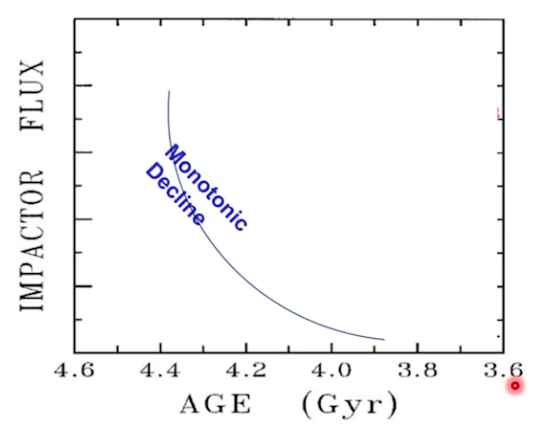
\includegraphics[width=0.8\textwidth]{LunarImpactFluxModelMonotonicDecline}
	\end{subfigure}
	\begin{subfigure}[t]{0.45\textwidth}
		\caption{When the first Lunar samples were dated using Uranium/Lead, we saw a spike instead, known as the Cataclysm, or Late Heavy Bombardment.}
		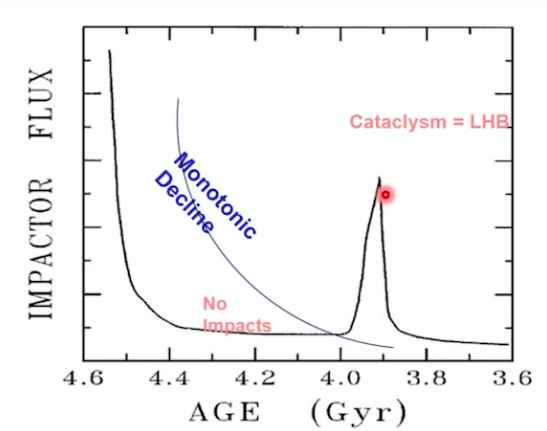
\includegraphics[width=0.8\textwidth]{LunarImpactFluxModelsWithLHB}
	\end{subfigure}
	\begin{subfigure}[t]{0.45\textwidth}
		\caption{Some investigators now believe there was a series of intense bombardments, with the LHB merely the last one}
		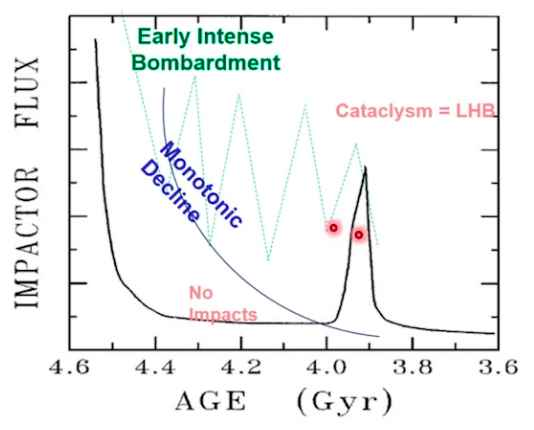
\includegraphics[width=0.8\textwidth]{LunarImpactFluxModelsEIBplusLHB}
	\end{subfigure}
	\begin{subfigure}[t]{0.45\textwidth}
		\caption{New understandings of Solar System Dynamics, plus younger material appearing in Lunar samples has given rise to a 4th scenario, the Sawtooth.}
		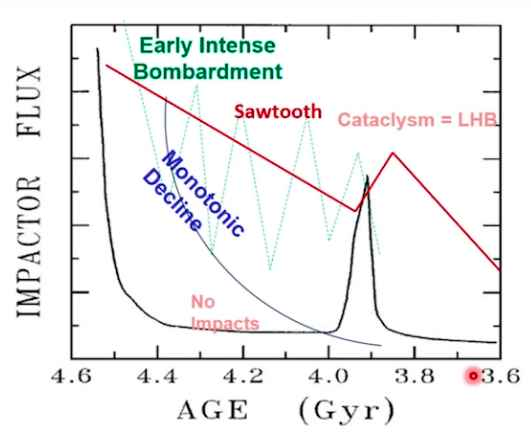
\includegraphics[width=0.8\textwidth]{LunarImpactFluxModelsNice}
	\end{subfigure}
\end{figure}

\begin{figure}[H]
	\caption[Importance of Lunar Impact Flux Models]{It is important to understand the Lunar Flux, because we start to see evidence for a cool early Earth (water and continents) and of life.}\label{fig:LunarImpactFluxModelsLife}
	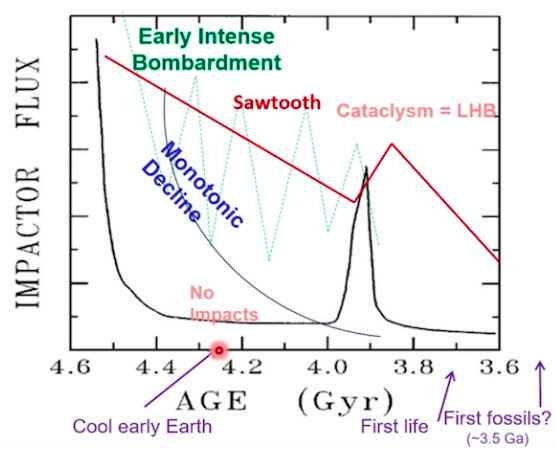
\includegraphics[width=0.8\textwidth]{LunarImpactFluxModelsLife}
\end{figure}

The Lunar Impact Flux allows us to constrain some of the evidence that we see in this early period. There are various ways to interpret the time-varying impact flux
\begin{itemize}
	\item Samples
	\begin{itemize}
		\item crystalline melts in Apollo samples
		\item crystalline melt casts in meteorites
		\item zircons
		\item lunar impact glass (Nicolle's speciality: the glasses retain a memory of the impact.)
	\end{itemize}
	\item Other
	\begin{itemize}
		\item crater counting
		\item stratigraphy
	\end{itemize}
\end{itemize}

Figure \ref{fig:TheCataclysm} shows the Lunar near side, showing that the ages of many of the features are around 4.9 Ga.
\begin{figure}[H]
	\caption[ Lunar near side]{ Lunar near side: U-Pb ages Stratigraphy; Crater counting; A15, A17 breccia; 40Ar/39Ar ages}\label{fig:TheCataclysm}
	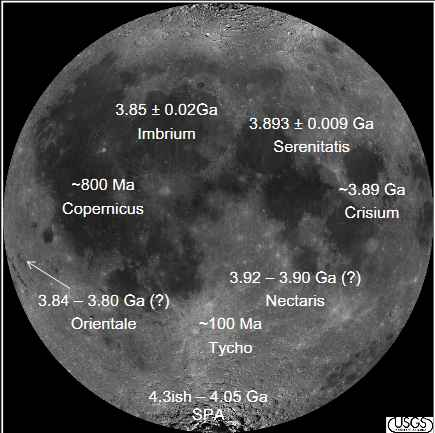
\includegraphics[width=0.8\textwidth]{TheCataclysm}
\end{figure}

\begin{figure}[H]
	\caption[Lunar meteorites]{Lunar meteorites. While there is no spike at 3.9Ga, there is little or no evidence of meteorites older than this date.}
	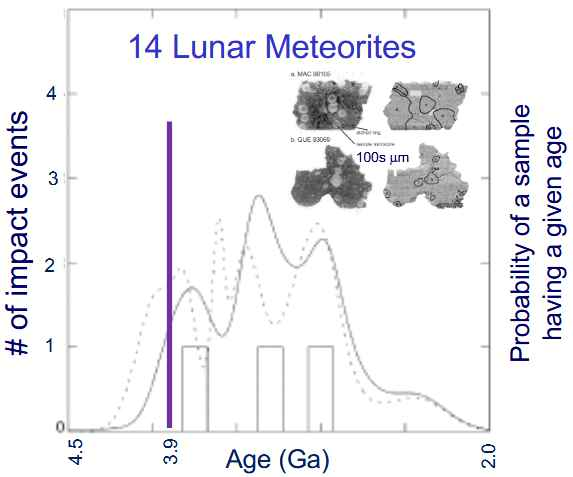
\includegraphics[width=0.8\textwidth]{LunarMeteorites}
\end{figure}

What could account for this cataclysmic event? Figure \ref{fig:nice:model} depicts the Nice Model, where the giant planets did not form in their current positions. When they reached a resonance they shook up the Kuiper Belt.

\begin{figure}[H]
	\caption{The Nice Model}\label{fig:nice:model}
	\begin{subfigure}[b]{0.3\textwidth}
		\caption{Early configuration, before Jupiter and Saturn reach a 2:1 resonance (JSNU)}
		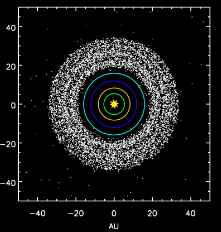
\includegraphics[width=\textwidth]{Nice1}
	\end{subfigure}
	\begin{subfigure}[b]{0.3\textwidth}
		\caption{Objects scatter into the inner Solar System after the orbital shift of Neptune (dark blue) and Uranus (lt. blue)}
		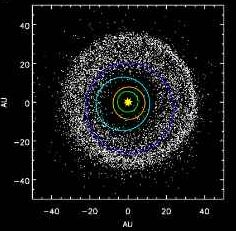
\includegraphics[width=\textwidth]{Nice2}
	\end{subfigure}
	\begin{subfigure}[b]{0.3\textwidth}
		\caption{Current-ishSolar System, after ejection of objects by planets (JSUN)}
		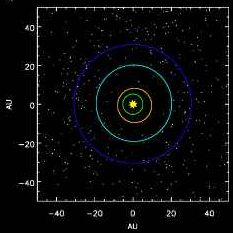
\includegraphics[width=\textwidth]{Nice3}
	\end{subfigure}
\end{figure}

But now we have very high resolution data from the Lunar Reconnaissance Orbiter--Laser Altimeter data and camera data. We also have new interpretations of the Apollo data, more data, and improved analytical techniques. Grange et al looked at some of the samples from 3.9 Ga--Figure \ref{fig:IsotopeRecalibrations}--and found they had roughly the same composition and the same age. They attribute all these sample to one event--Imbrium--Figure \ref{fig:TheCataclysm}. The proposed that Imbrium material contaminated the entire near side of the Moon, hence all the Apollo landing sites.
\begin{figure}[H]
	\caption{Isotope Recalibrations}\label{fig:IsotopeRecalibrations}
	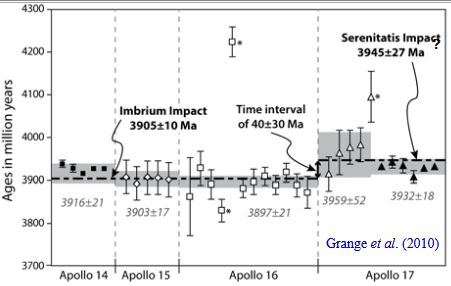
\includegraphics[width=0.8\textwidth]{IsotopeRecalibrations}
\end{figure}

Comparing Figures \ref{fig:UpdatedBasinAges} and \ref{fig:TheCataclysm}, we see that we are now attributing a much wider variation to the ages.
\begin{figure}[H]
	\begin{center}
		\caption[Updated Basin Ages]{Updated Basin Ages(based on new calibrations and superpositioning of ejecta blankets from orbital data). Imbrium’sage is based on Apollo 14 and Apollo 15 samples, whose geologic provenance is not well-established.}\label{fig:UpdatedBasinAges}
		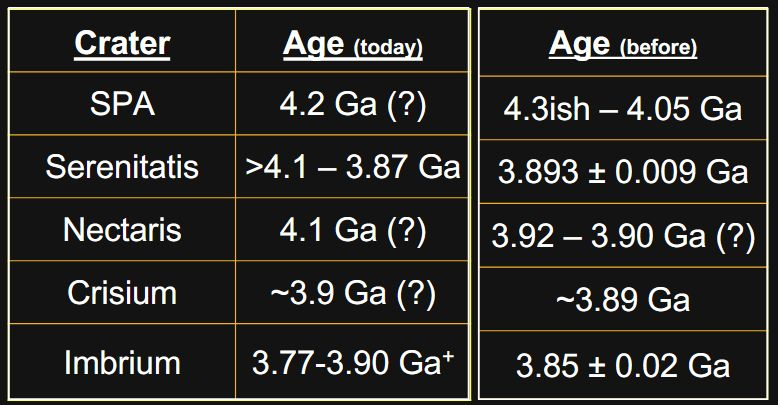
\includegraphics[width=0.8\textwidth]{UpdatedBasinAges}
	\end{center}
\end{figure}

More recently the Gravitometric Data from the \gls{gls:GRAIL} satellite--Figure \ref{fig:GrailData}-- has found
\begin{itemize}
	\item Multiple new basins w/>300km diameters
	\item 6 known basins with D>200km larger than previously measured, hence
	\item crater size frequency distribution needs to be recalibrated and the impact flux changes
\end{itemize}

\begin{figure}[H]
	\caption{Grail Data}\label{fig:GrailData}
	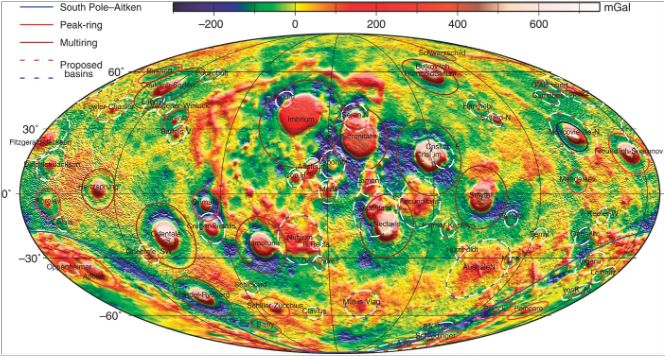
\includegraphics[width=0.9\textwidth]{GrailData}
\end{figure}

We now have evidence for Archaen impacts--Figure \ref{fig:ArchaeanImpactsOnEarth}--so the Late heavy Bombardment lasted longer than we thought. Multiple impact spherule layers from large distal impacts between 3.5 and 3.2 Ga
 
\begin{figure}[H]
	\caption{Archaean Impacts On Earth}\label{fig:ArchaeanImpactsOnEarth}
	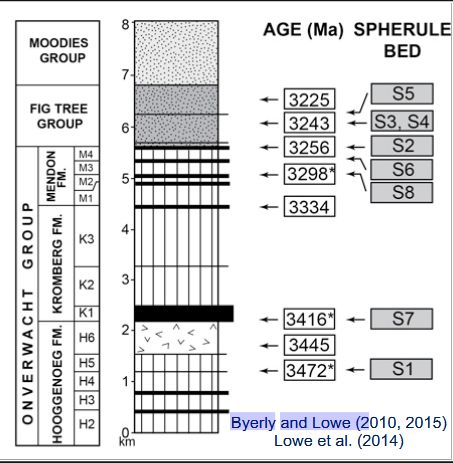
\includegraphics[width=0.9\textwidth]{ArchaeanImpactsOnEarth}
\end{figure}

We have more sensiive instruments and can look at smaller samples than before:
\begin{itemize}
	\item Apollo 16 impact breccia U-Pbage: large event at $4.22\pm0.01Ga$ 
	\item Apollo 16 melt 40Ar–39Ar ages: $4.21\pm0.05$ Ga and  $4.29\pm0.04$ Ga
	\item Lunar zircon heating events w/U–Pbages:  $4.3\pm0.01$,  $4.2\pm0.01$, and  $3.9\pm0.01$ Ga
\end{itemize}

This is pointing to impacts before 3.9 and after 3.9, so that narrow cataclysmic spike probably didn't happen.

\begin{figure}[H]
	\caption{Lunar Flux as a function of Age}\label{fig:LunarFlux}
	\begin{subfigure}[t]{0.30\textwidth}
		\caption{Histogram showing probability of sample having a given age.}
		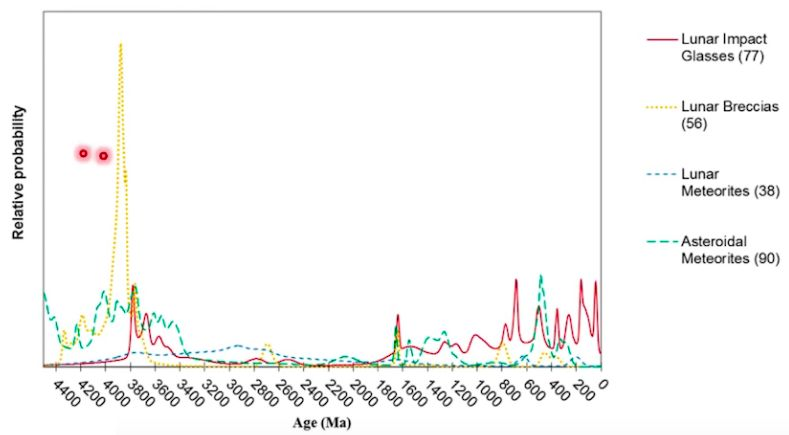
\includegraphics[width=0.8\textwidth]{LunarFlux0}
	\end{subfigure}
	\;
	\begin{subfigure}[t]{0.30\textwidth}
		\caption{Suppressing the Imbrium contamination gives more of a sawtooth}
		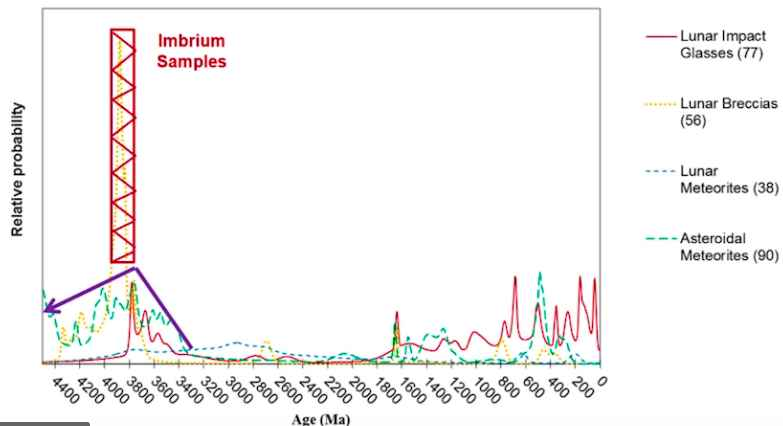
\includegraphics[width=0.8\textwidth]{LunarFluxWithoutImbrium}
	\end{subfigure}
	\;
	\begin{subfigure}[t]{0.30\textwidth}
		\caption{Impacts relatively quiet during Great Oxidation Event, and also during first whiffs of oxygen on earth. Has bombardment picked up on right, or is it just better preserved?}
		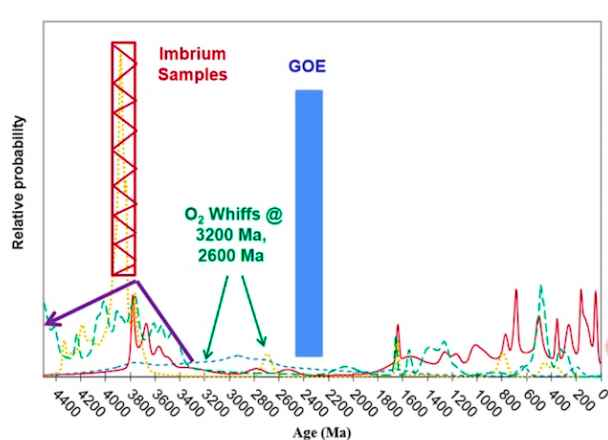
\includegraphics[width=0.8\textwidth]{LunarGOE}
	\end{subfigure}
\end{figure}


Interesting things are happening on Earth at this time.

\begin{itemize}
	\item C isotope evidence for life:
	\begin{itemize}
		\item  $>4.0$ Ga, Biogenic carbon in zircons (Bell et al. 2015)
		\item 3.95 Ga, Canada (Tashiroet al. 2017)
		\item 3.85 Ga, Akilia, Greenland (Mojzsiset al.1996)(though highly contested in the literature)
		\item 3.8 Ga, Isua Greenland (Schidlowski, 1988)
	\end{itemize}
	\item Fossil evidence for life: 
	\begin{itemize}
		\item 3.77 Ga, marine hematite tubes(Dodd et al. 2017)
		\item 3.48 Ga, terrestrial palisade fabric
	\end{itemize}
\end{itemize}

Early Life on Earth

\begin{itemize}
	\item Impacts were not very frequent but were prolonged (~4.1 to 3.2 (or younger) Ga)
	\begin{itemize}
		\item No impact frustration(Maher and Stevenson, 1988)
		\item No impact sterilization(Sleep et al. 1989; Nisbetand Sleep, 2001)
		\item A cool early Earth(Wilde et al., 2001; Watson and Harrison, 2005)
		\item Delivery of CHONPS(e.g., amino acids, sugars)
	\end{itemize}
	\item Impacts did affect life but still it persisted
\end{itemize}

\section{Likely Environments for Studying Origins of Life}

\subsection[Likely Environments for Studying Extremophiles]{Likely Environments for Studying Extremophiles-- Nancy Merino}

One of the research areas I think about is the likely environments for studying origins of life.
In order to do this, we have to first understand
what it might have been like on Early Earth billions of years ago.
Then, once we have an idea of that, we can look around on Earth today for similar environments and search for life.

The idea is that we can find clues about early life within modern day life --much like how your own life is a reflection of your own personal history and family's history.
Life probably started
around 4.4 to 3.8 billion years ago. The origins of life is still
a highly debated topic,
so the range still covers
billions of years.
This is what's shown here
in the timeline of Earth's history,
from its formation
about 4.5 billion years ago
to the current times--Figure \ref{fig:LifeProbablyStarted}.


\begin{figure}[H]
	\caption[Life probably started between 4.4 to 3.8 billion years ago]{Life probably started between 4.4 to 3.8 billion years ago (Ga) \cite{domagal2016astrobiology}} \label{fig:LifeProbablyStarted}
	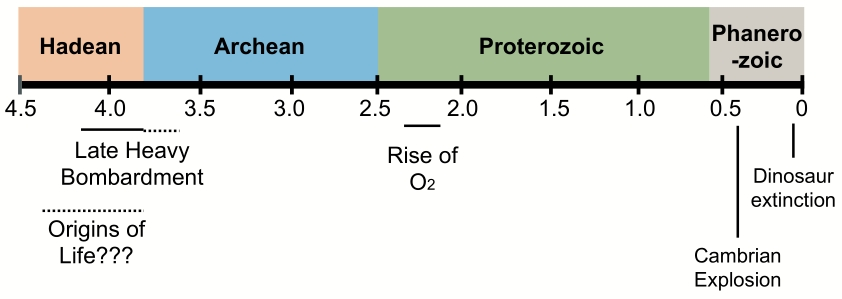
\includegraphics[width=0.9\textwidth]{LifeProbablyStarted}
\end{figure}

There are four different eons of Earth,
known as the Hadean, Archean
and Proterozoic and Phanerozoic Eons.
These are all major time periods
marked by drastic changes
in the Earth's environment.

It's believed that life originated
some time during the Hadean
and Archean Eon.
And, during this time,
there is also probably a lot of comet
and meteorite impacts -
and this is what's known as
the "Late Heavy Bombardment."
These comets and meteorite impacts
would have influenced
the Early Earth environment
because there were just so many of them.
It is one reason why some scientists think
that life may not have started
during the Hadean Eon
because it was extremely hot
and probably inhospitable for life.
Figure \ref{fig:HadeanInhospitable} is an image showing
what it might have looked like on Earth
during the Hadean Eon.
But, this is still a highly debated topic
because we don't have
a really good rock record.
However, we do know that Early Earth
was probably an extremely hot
environment.
\begin{figure}[H]
	\caption[Earth during the Hadean Eon was probably very inhospitable]{Earth during the Hadean Eon was probably very inhospitable for life} \label{fig:HadeanInhospitable}
	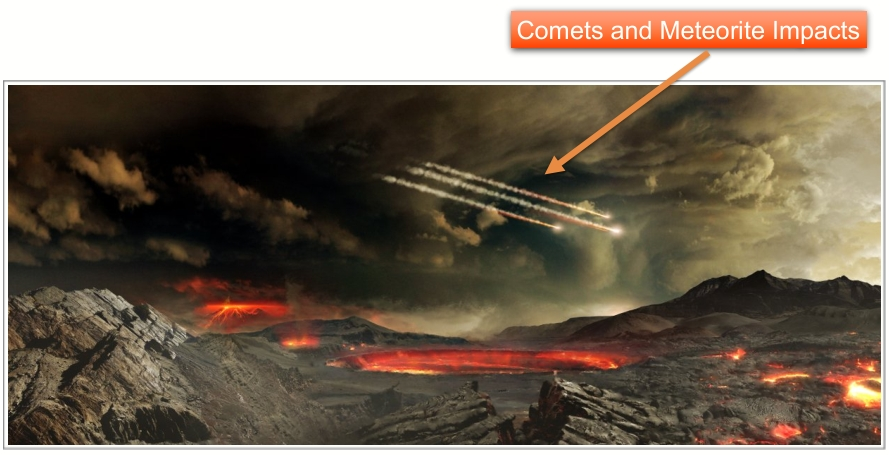
\includegraphics[width=0.9\textwidth]{HadeanInhospitable}
\end{figure}

There were also magma oceans.
So, instead of water,
the Early Earth oceans
were made of magma.
These magma oceans started
because of several reasons,
\begin{itemize}
	\item one of which is comet and meteorite impacts, which heated up the surface of the Earth.
	\item Another is tidal heating, which has influences from how close the Moon is to the Earth.
	\item Another is core formation,
	where comet and meteor impacts
	will deposit metals
	onto the surface of the Earth,
	and this will begin sinking
	towards the inner layers of the Earth,
	helping to form the Earth's core.
	This process is known
	as "plate tectonics"--Figure \ref{fig:PlateTectonics}.
\end{itemize}

\begin{figure}[H]
	\caption{Plate Tectonics could have started
		as early as 3.8 billion years ago}\label{fig:PlateTectonics}
	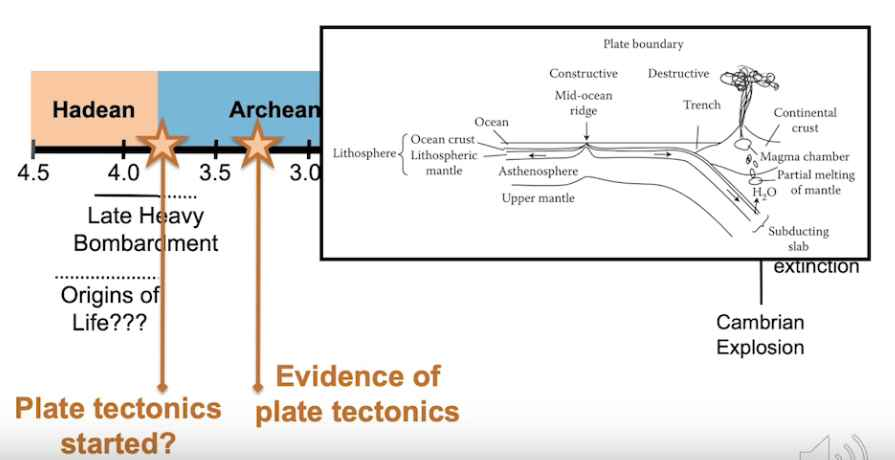
\includegraphics[width=0.8\textwidth]{PlateTectonics}
\end{figure}
So, Earth has a thin surface layer,
which is cracked and can move around.
This is the reason for earthquakes,
and it is also essentially
the recycling of Earth's surface
with the inner parts of the Earth.
This process could have started
as early as 3.8 billion years ago
and is definitely occurring
around 3.2 billion years ago.
This motion most likely helped make
the Early Earth environment
more favorable for life
by helping to cool down the Earth.

In addition to influencing
the origins of life,
plate tectonics also influenced
the evolution of life
through the creation
and movement of continents.
A necessary requirement
for plate tectonics is water.

\begin{figure}[H]
	\caption[Formation of Oceans]{Before plate tectonics really got started,
		oceans probably started to form
		during the Hadean Eon.}\label{fig:FormationOfOceans}
	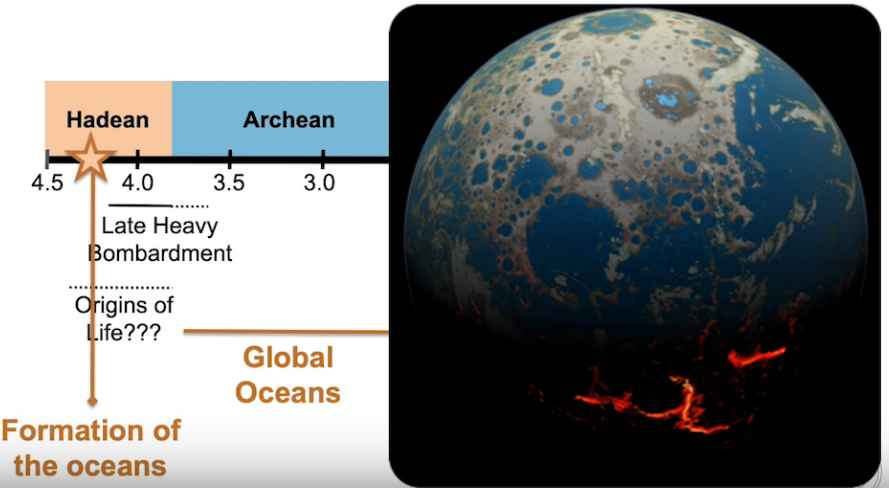
\includegraphics[width=0.8\textwidth]{FormationOfOceans}
\end{figure}
Before plate tectonics really got started,
oceans probably started to form
during the Hadean Eon.
But, it is not until the Archean Eon
that there are really global oceans
covering the surface of the Earth.
This water didn't just come from nowhere
and there were at least
three sources of water.

\begin{itemize}
	\item One is from plate tectonics influencing the amount of water on Earth's surface.

	\item Another source is from volcanoes, which were very active at this time
	and would have helped the conversion of water vapor into liquid.

	\item The third source is from delivery by comets and asteroids,
	which are rich in ice.

\end{itemize}

Water is definitely one of the most
important substances
at this time to help start life
and is really the main criteria
for life on Earth.
For example,
water plays an important role
in the stability and dynamics
of life's major compounds -
like proteins and \gls{gls:DNA}.

Life took hold on Earth during the Archean Eon--Figure \ref{fig:Chemolithoautotrophs}. There were a mix of things going on
at this time,
which made it possible.
This includes a not so hot environment,
mainly due to the cooling of Earth
by plate tectonics and other processes -
the formation of a global ocean
and the collection of the necessary
ingredients on Early Earth
to actually build a cell-like shape.
\begin{figure}[H]
	\caption{Life took hold on Earth during the Archean Eon} \label{fig:Chemolithoautotrophs}
	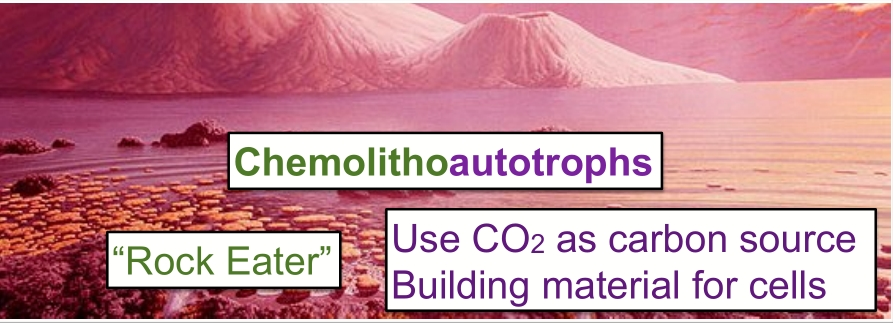
\includegraphics[width=0.9\textwidth]{Chemolithoautotrophs}
\end{figure}



However, life during the Archean Eon
had to survive without oxygen.
The atmosphere probably had nitrogen,
carbon dioxide, water
and some amounts of sulfur,
methane and ammonia.
The atmosphere during this time
is actually still highly debated,
but scientists agree
that Early Earth atmosphere
during this time had no free oxygen.
This atmosphere is very much different
from today's atmosphere,
which has 21 percent oxygen.

The earliest life-forms were probably
what we call "chemolithoautotrophs."
The first part of this word
is "chemolitho,"
and that's short for chemolithotroph.
This is Greek for "rock-eater,"
and it means
that the earliest life-forms
probably used inorganic compounds -
for example, iron or sulfur
to get energy.
The second part of this word
is "autotroph."
This means that the first cells
used carbon dioxide for getting carbon.

Carbon is the necessary building material
for our cells,
And so, the Archean Eon essentially had
all the necessary ingredients for life.

We know that life probably took hold
in the Archean Eon
because there is evidence of life
in the rock record.
The first likely signs of life
in the rock record
starts around 3.5
to 3.3 billion years ago.
Figure \ref{fig:EvidenceOfLife} depicts a rock in Western Australia,
which dates back to that time.

\begin{figure}[H]
	\caption[Archaean microfossil
	from a rock in Western Australia]{Here is an image showing a microfossil
		from a rock in Western Australia, which dates back to that time.}\label{fig:EvidenceOfLife}
	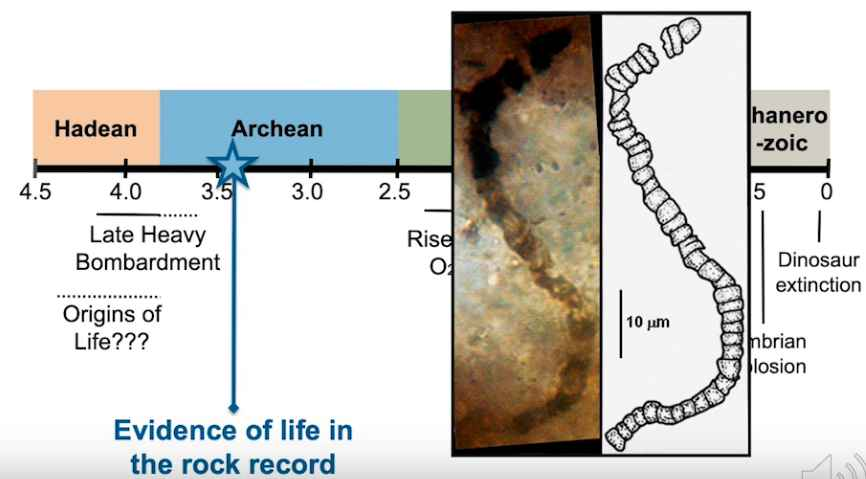
\includegraphics[width=0.8\textwidth]{EvidenceOfLife}
\end{figure}
Now we have an idea
of what Early Earth was like,
in now - in modern times -
we are faced with the task
of deciphering the origins
and evolution of life.
How can we think about early life
right now?
To build on top of that,
how can we think about life
on other planetary bodies?
And, modern day Earth
actually has some answers for us.

\begin{figure}[H]
	\caption[A selection of Extreme Environments]{The Earth today is covered
		with many modern-day analogues
		for Early Earth
		and other planetary bodies.}\label{eq:ExtremeEnvironments}
	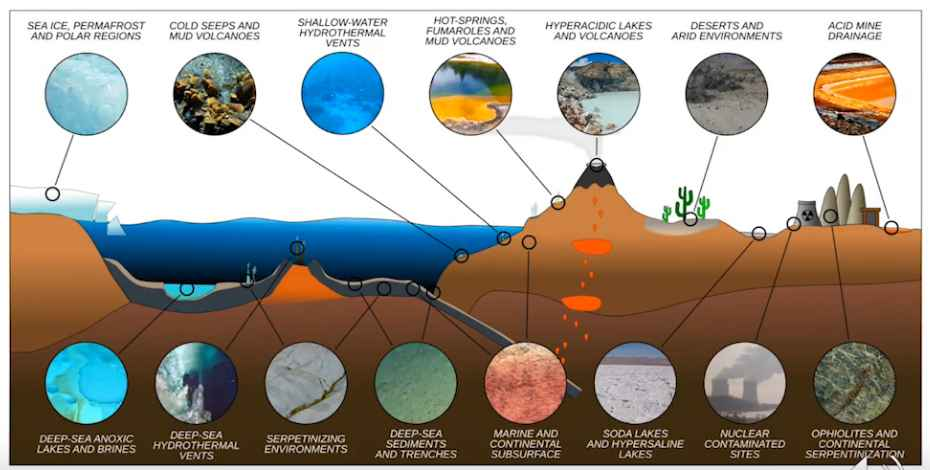
\includegraphics[width=\textwidth]{ExtremeEnvironments}
\end{figure}
The Earth today is covered
with many modern-day analogues
for Early Earth
and other planetary bodies.
These are all extreme environments.
This image here shows the locations
where microorganisms
have been discovered
all the way from the deep parts
of the ocean
to the Arctic and to volcanoes.

All of these environments
have some kind of extreme component
that requires microbes to have
the necessary adaptations to survive.
So, by studying these environments,
it allows scientists to understand
how microbes can adapt to
extreme environments
and how they might have lived
on Early Earth,
and the potential for life
on other planetary bodies.
Many microbes have been identified
in these extreme environments,
and the microbes that can survive
under extreme conditions
are known as "extremophiles."

Extremes include temperature, pH,
salinity, pressure,
desiccation - or extreme dryness -
and radiation tolerance.
Here are five microscope images
of microbes that can survive
under the most extreme conditions,
and these are the current record holders.

\begin{figure}[H]
      \caption[Five Extremophiles]{Here are five microscope images
      	of microbes that can survive
      	under the most extreme conditions,
      	and these are the current record holders}\label{fig:Extremophiles}
      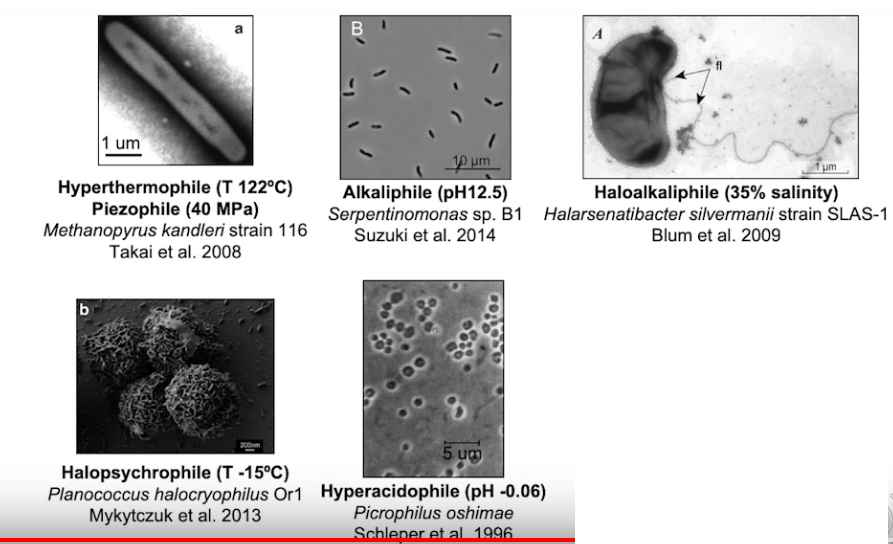
\includegraphics[width=0.8\textwidth]{Extremophiles}
\end{figure}

So, for example,
Methanopyrus kandleri can grow
at temperatures
up to 122 degrees Celsius -
so this is way above boiling water.
But, because of high pressure,
the water where this microbe
is naturally found does not boil -
and so, this microbe can survive
both high temperatures and high pressure.
And, because it can survive
multiple extremes,
it's also known as
a "polyextremophile."

\begin{figure}[H]
	\begin{center}
		\caption{Life on Earth could potentially survive
		under even more extreme conditions}\label{fig:EarthLifeExtremes}
		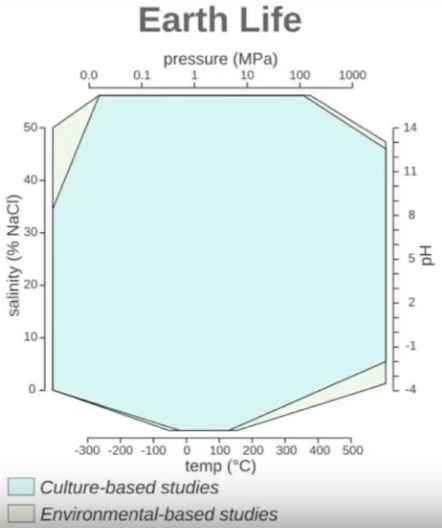
\includegraphics[width=0.8\textwidth]{EarthLifeExtremes}
	\end{center}
\end{figure}
Life on Earth could potentially survive
under even more extreme conditions.
Figure \ref{fig:EarthLifeExtremes} is showing
temperature, pH,
pressure and salinity on different axes.
The temperature ranges from minus 300
to 500 degrees Celsius,
the pH ranges from minus 4 to 14,
the pressure ranges from zero
to 1000 megapascals
and salinity ranges from zero
to 50 percent.
The minimum and maximum
for each parameter
is plotted for life on Earth,
and so we can see the space
in which life on Earth occupies.
Now, when we look at all the known
extreme environments on Earth,
we can see there is potential
to push the boundaries of life
on Earth even further.
For example, the maximum temperature
life can grow at
is currently 122 degrees Celsius,
but Earth's environments can reach
to much higher temperatures.
It may not be possible for life to survive
at 400 degrees [Celsius],
but there is potential for microbes
to survive a bit hotter temperatures
than 122 degrees [Celsius].
So, there are many unexplored
regions of Earth
where new microbes
have yet to be discovered.

\begin{figure}[H]
	\caption{What About Other Planetary Bodies?}\label{fig:WhatAboutOtherPlanetaryBodies}
	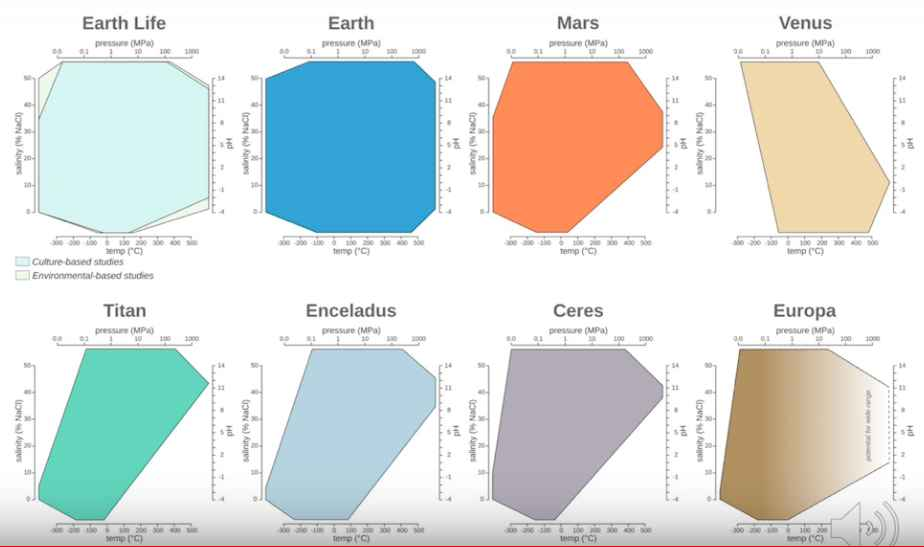
\includegraphics[width=\textwidth]{WhatAboutOtherPlanetaryBodies}
\end{figure}
But, what about other planetary bodies?
When we look at
the environmental conditions
on the planets Mars, Venus
and the dwarf planet Ceres,
as well as the icy moons Titan,
Enceladus and Europa,
we can see that there are some portions
of those planetary bodies
which match up to the environmental
conditions on Earth.

So, by studying the modern-day analogues
on Earth,
we can further understand life itself
and also explore life in the Universe.


\subsection{Cuatro Ci\'enegas Special Feature}

This is a short film about the people and places of the Cuatro Ci\'enegas Basin in Coahuila, M\'exico.\footnote{This is the transcript from the video, with a few small edits.} The Cuatro Ci\'enegas Basin - its water and microbial, plant and animal communities -
are a treasure of M\'exico. All of this unique life has been uncovered through the work of Mexican scientists with inte\gls{gls:RNA}tional collaborations. This work makes possible a deeper understanding of the history of all of life on earth.

\begin{figure}[H]
	\caption{The Cuatro Ci\'enegas Basin} 
	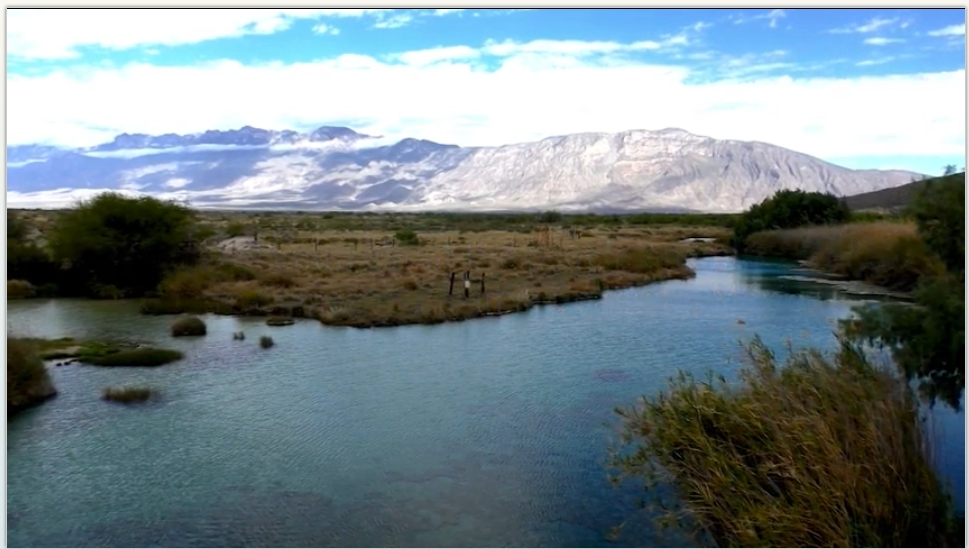
\includegraphics[width=0.9\textwidth]{CuatroCienegas1}
\end{figure}

\subsubsection{Introduction: Valeria Souza}

My name is Valeria Souza. I work as a researcher at UNAM - the National University of Mexico, that is a very large university. This is probably the most important site
that we have in the world right now to understand the origin of diversity. This place has an amazing geology that you can see just in front of you.\cite{souza2018lost}

\begin{figure}[H]
	\caption{We have that kind of tsunami of rocks} 
	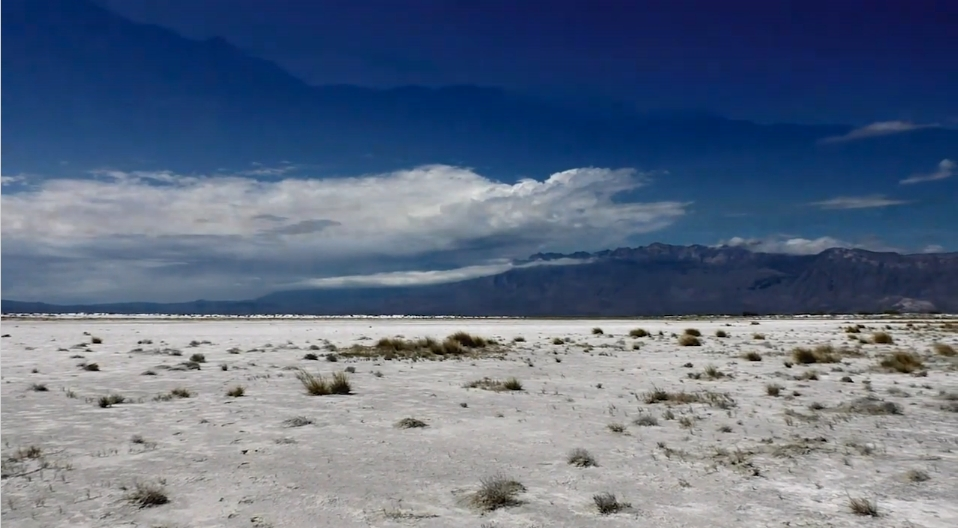
\includegraphics[width=0.9\textwidth]{CuatroCienegas2}
\end{figure}

We have that kind of tsunami of rocks that uplifted, because the mountain
that is over that edge is like an arrow. It has an active fault
with magma underneath. And, it's pushing all the marine sediments that are from this valley up and then it's flipped and makes a heart shape -- a 3,000 meter mountain.

So, all this amazing geology is an explanation of why Cuatro  Ci\'enegas is a singularity -- because these marine sediments store the conditions of the ancient sea. They store the magma that is rich in sulfur, that takes us all the way back to the Archean, and it stores the minerals that formed in sand. These minerals are very old.

Also, it is a sediment that is devoid of the most basic element for life, that is, phosphorus. So, this site is amazingly poor in phosphorus, and that makes for a very
skewed stoichiometry. Most of life now cannot live in a skewed stoichiometry -- we need 60 nitrogens for each phosphorus. Here, we have 100 nitrogens - at least - for each phosphorus, in some places 200 nitrogens for each phosphorus.

So, how they can make basic things, such as ribosomes or \gls{gls:DNA}, is because they are really good at stealing phosphorus from anybody else, including rocks. So, they have an amazing array of strategies to deal with the lack of phosphorus, and they did that since the Archean.

So, here we have stromatolites and microbial mats, whose ancestry goes back
to the Precambrian in some cases. And, we are going to a site where we think we have the boundary between the Archean and the Precambrian\footnote{Should this be Proterozoic?}. Since this is a blue pool, we are talking about the moment where animals turned the planet blue, and that was in the Ediacaran in the late Precambrian.

\subsubsection{Microbial Mats: Maria Kalambokidis}
My name is Maria Kalambokidis, and I'm an intern for a year, working in Valeria's lab in UNAM, in the Department of Evolutionary Ecology. And, right now, we're at Pozas Azules, at the site of the Archaean domes. 

\begin{figure}[H]
	\caption[A microbial mat showing the activity of  methanogens]{A microbial mat that created a bubble through the activity of  methanogens} 
	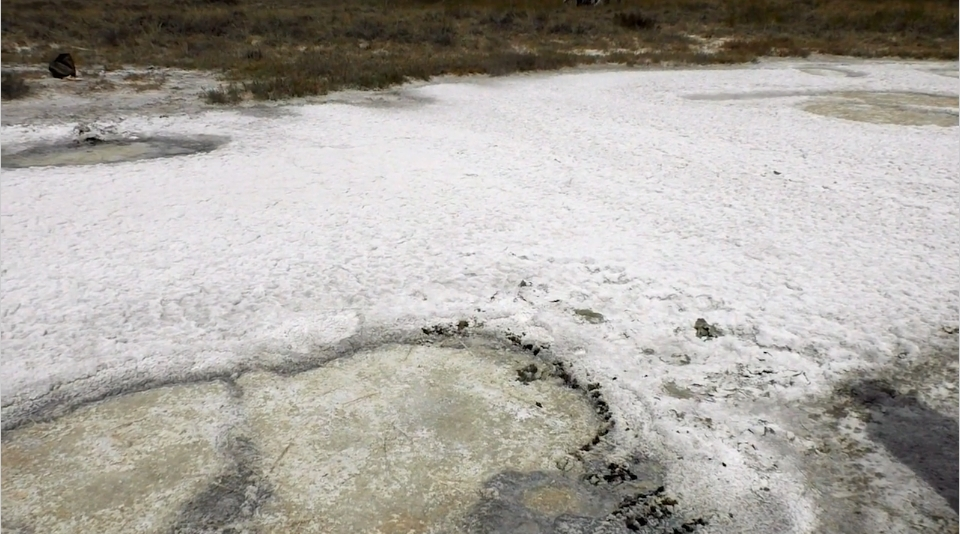
\includegraphics[width=0.9\textwidth]{CuatroCienegas3}
\end{figure}

So, here you have a microbial mat that created a bubble through the activity of the methanogens. It created a bubble and then it eventually burst, creating this perimeter. So, we sampled the microbial mats that are still present there. And, right now, they're hidden beneath the salt crust, because it's so dry. My research is looking at the evolutionary resilience of the microbial mats at Cuatro i\'enegas.

So, the microbial mats create a codependent community where each layer is sort of representing the history of metabolisms on Earth--Figure \ref{fig:MicrobialMatDetail}. So, you start with methanogens, 
which create nutrients for the next layer of sulfur-oxidizing bacteria, all the way up until photosynthesis. So, through this community, they've become really dependent on each other and they evolve together, creating a really resilient community in Cuatro  Ci\'enegas that has existed for many millennia.

\begin{figure}[H]
	\caption{The microbial mats create a codependent community}\label{fig:MicrobialMatDetail}
	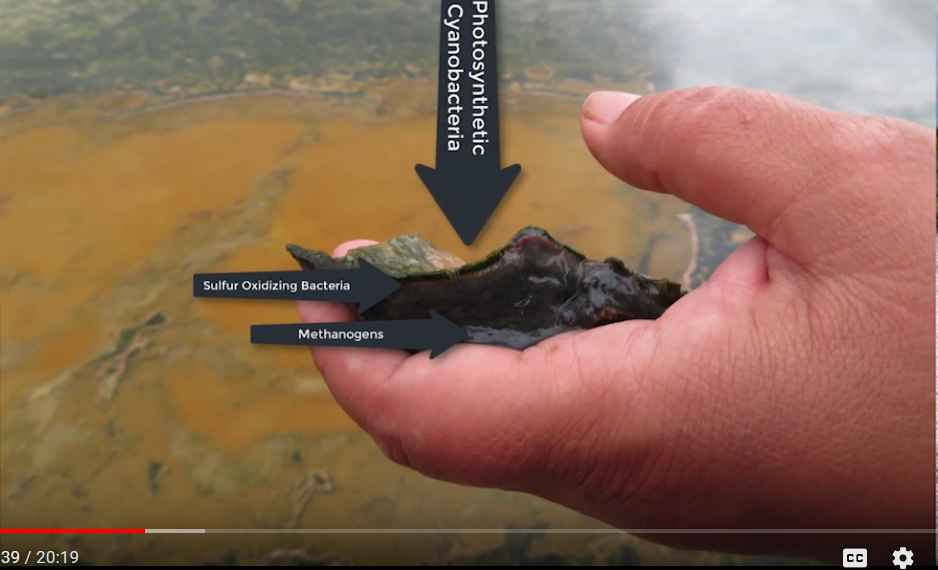
\includegraphics[width=0.8\textwidth]{MicrobialMatDetail}
\end{figure}

I was interested in the microbial mats because they're evolutionary resilient
and they've existed so long here, but also because they've existed in an environment that many other organisms couldn't exist. For example, a really low nutrient content, in particular, low in phosphorus, which is thought to be necessary for the building blocks of life.

So, they've existed for so long, they're able to exist in extreme environments. Therefore, it creates a sort of living laboratory of organisms that are alive today and indicative of communities that existed long ago. So, in origin of life research and in astrobiology, usually you're looking for signs of life - like biosignatures on another planet, or you're breaking open old rocks to see if there are compounds indicative of life. But, in Cuatro  Ci\'enegas, and in these mats, we think that we have the organisms that formed the same communities that existed long ago.  So, as a biologist, it's really exciting to actually be able to study it alive today.

\subsubsection{Churince System, Intermediate Lagoon: lost due to unmanaged surface and groundwater extraction}
The big questions why so many species on planet Earth or in this place
???the history of survival???

The origin of life was probably very easy.

The origin of life was probably ??????
millions of ways possible???

On this planet, life survived???

???? the rocks
and transformed all of the minerals.???
\subsubsection{Dra. Gabriela Olmedo Alvarez}
My name is Gabriela Olmedo-Álvarez, and I work at Cinvestav: ''center of research for advanced studies.'' I'm in Mexico, right in the middle of Mexico - in Irapuato. I'm the director of Cinvestav in Irapuato, although I am also a researcher. And, I've been working for 15 years, close to Valeria Souza, in trying to decipher what are the keys that allow so much diversity of microorganisms inhabit these places.

\begin{figure}[H]
	\caption{Pond with few nutrients but plenty of life.} 
	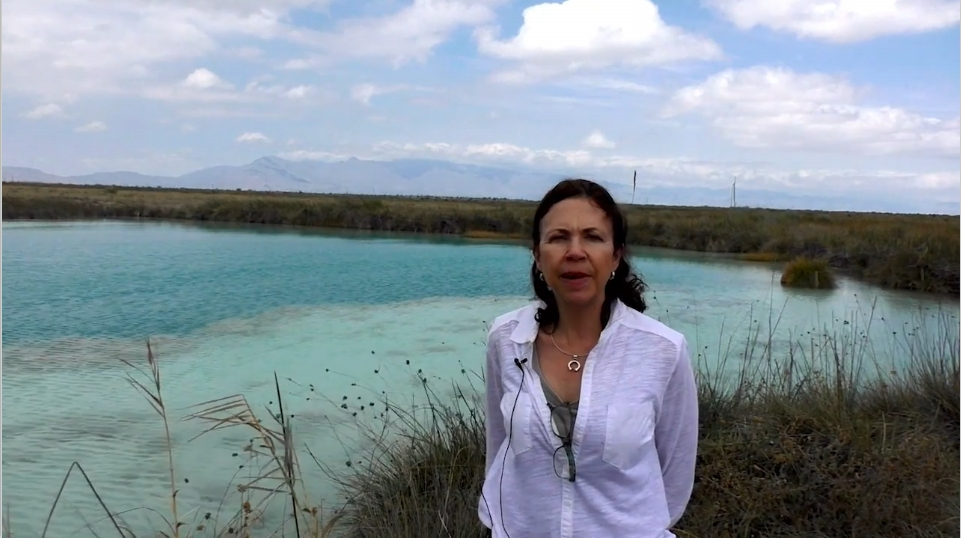
\includegraphics[width=0.9\textwidth]{CuatroCienegas4}
\end{figure}

And, if you are looking at the pond behind me - that's a beautiful pond, and it looks like it doesn't have much, because it doesn't have a lot of nutrients. That is why it's so interesting - it doesn't have nutrients, but it has lots of different bacteria, and has evidence of very old life.

It also has these stone-like things that are stromatolites. Stromatolites are evidence of the first types of life on the planet, but here they are still alive. They are still, you know, blooming, and it's very interesting because these are very, very old types of life. And, that is possible precisely because there are no nutrients. So, other larger things
cannot compete with it, and that allows these to remain for centuries and millions of years.


But if we walk just a few meters away, maybe just 200 meters, we'll find a very different scenery. We'll find these very salty crusts, and these salty crusts are full of life also - a very special life with lots of salt and with a low pH. So, it's a weird life that we do not understand, and that's sort of one of the focuses that we have for this trip - to be able to sample what things are living there. And, we'll take them to the lab to figure out how some bacteria or archaea can live with these very, very extreme environments.

\begin{figure}[H]
	\caption[These salty crusts are full of life also]{These salty crusts are full of life also - a very special life with lots of salt and with a low pH.} 
	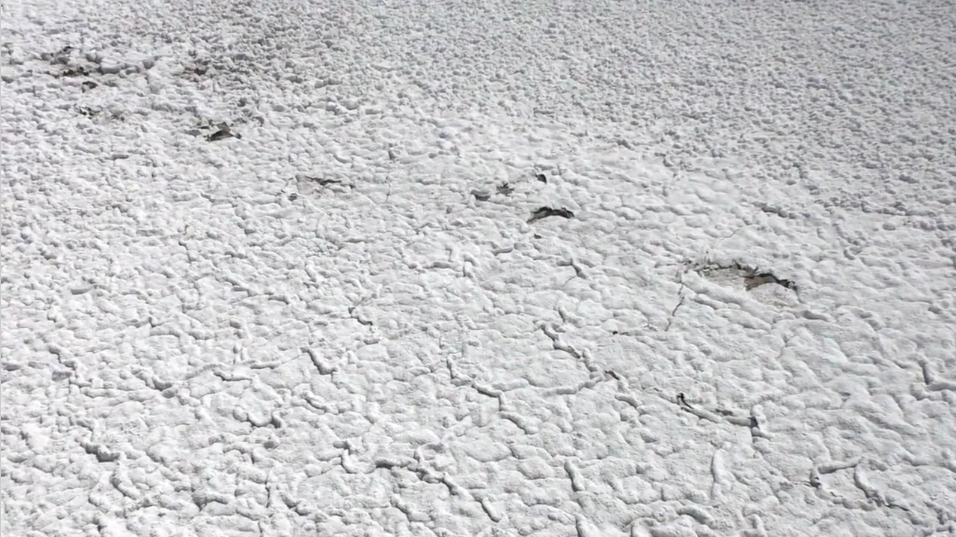
\includegraphics[width=0.9\textwidth]{CuatroCienegas5}
\end{figure}

\subsubsection{Pozas Rojas: Valeria Souza}

In the system called ''Pozas Rojas'', because these ponds are fluctuating environments, they get very saline in the summer because the water evaporates. It is deep water, not rain water, so each one becomes a more vivid color than in winter, where water doesn't evaporate as much -- so they get like the juiciness concentrated in the summer.

\begin{figure}[H]
	\caption{PosasVS}\label{fig:PosasVS}
	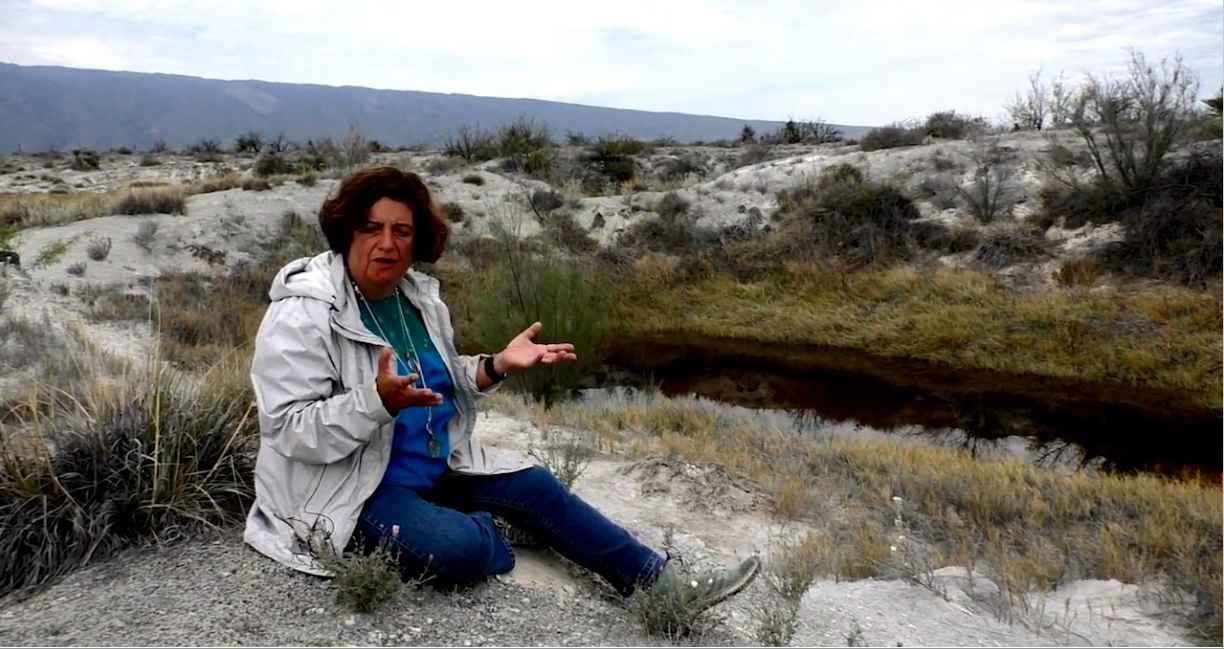
\includegraphics[width=0.8\textwidth]{PosasVS}
\end{figure}

The life that lives here is very diverse - there's microbial mass that we have sequenced.

\begin{figure}[H]
	\caption[The life that lives here is very diverse]{The life that lives here is very diverse - there's microbial mass that we have sequenced.}\label{fig:PosasBiodiversity}
	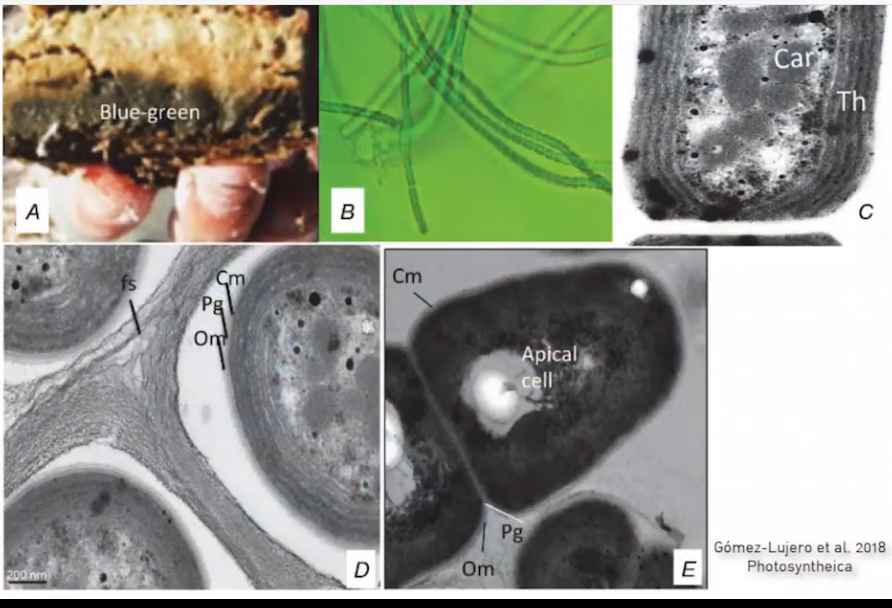
\includegraphics[width=0.8\textwidth]{PosasBiodiversity}
\end{figure}

There's a very large biodiversity and there are like islands. There are nine small islands of these tiny \gls{gls:poza}s and a big lagoon.

\begin{figure}[H]
	\caption{There are nine small islands of these tiny \gls{gls:poza}s and a big lagoon.} 
	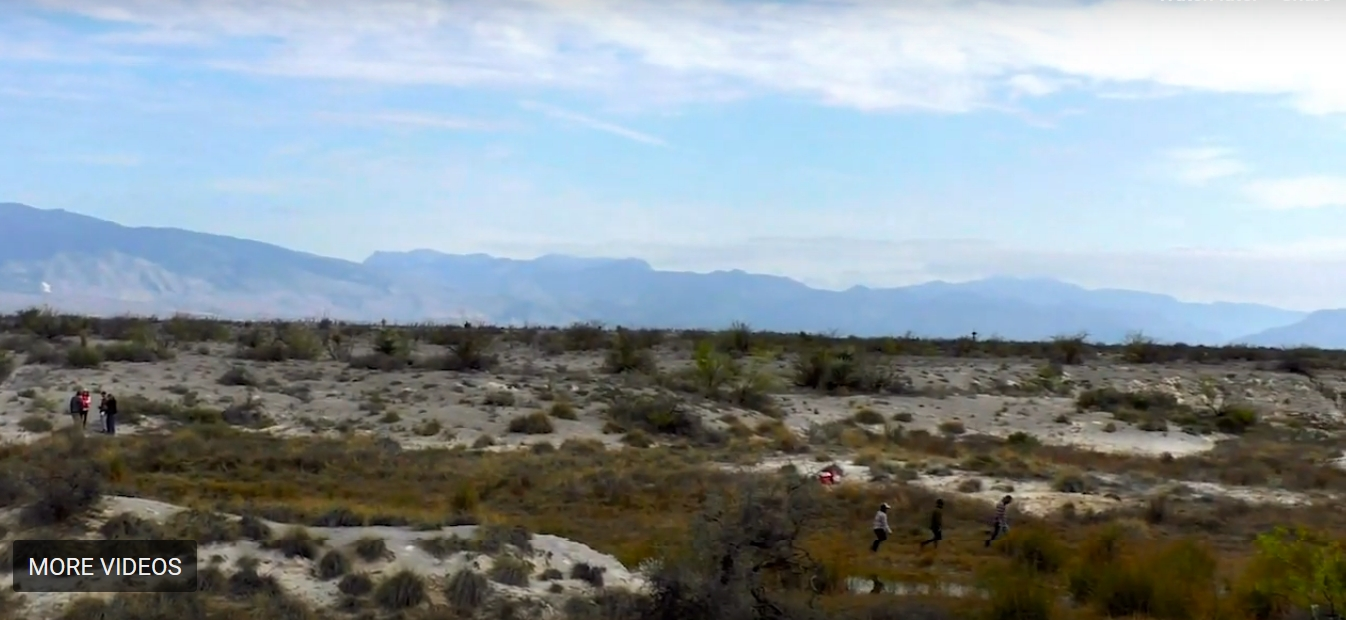
\includegraphics[width=0.9\textwidth]{CuatroCienegas7}
\end{figure}

So, you can compare the diversity in each one of them separately and then the big \gls{gls:poza} in the middle. But, this was perturbed by a hurricane in 2010 and it became a complete lake, all of its... It kind of drained all the nutrients and all the water from the... east side of the valley. The biology changed because the \gls{gls:poza}s became connected 
with the lake water, and also the nutrients changed. It was - before the hurricane - it was the site with less phosphorus. Now, it is a site that nearly has a balance of stoichiometry. So, it is very interesting how the life got habituated to this richer environment. What is even more interesting is that what was a very primitive site it became a more Holocene site.

For example, the Vibrio that lives here, they didn't radiate since the Holocene in Cuatro  Ci\'enegas, which is at the same time as the fishes came from the R\`io Bravo shelf. So, they are very interesting, and they are always changing, and that makes us really happy --and we are following their change. So, I'm sure that the deep aquifer still has the deep, ancient bacteria. It shows that the lake that shaped here, that came here, brought newer creatures from everywhere that were bacteria more used to nutrients. And, maybe there are pockets of nutrients in different parts of the valley.

What makes Cuatro  Ci\'enegas unique is precisely the lack of nutrients. Maybe they are going to become - each time that we sample - more and more imbalanced and return to their ancient selves. But, it will take time.

\subsubsection{Jorge Valdivia}

My name is Jorge Valdivia, and I am a full-time professor at the Universidad Nacional Aut\'onoma de M\'exico. [...] of my doctoral studies in the Cuatro  Ci\'enegas valley. I was working with the genus Bacillus and the project was focused on knowing the relationship that existed between the number of copies of the ribosomal operon and with the available phosphorus.\cite{valdivia2016variability}
\begin{figure}[H]
	\caption[Variability of the r\gls{gls:RNA} operon copy number]{Variability of the r\gls{gls:RNA} operon copy number in the Bacillus diversity from the Cuatro  Ci\'enegas basin} 
	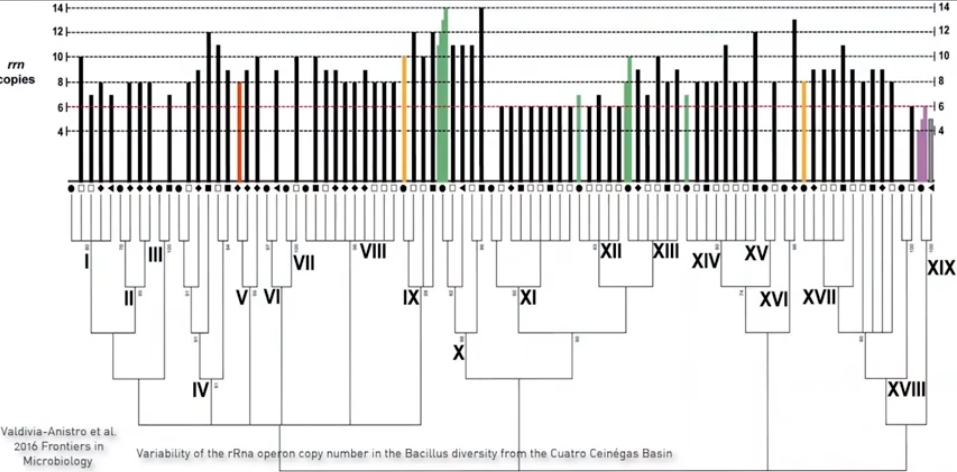
\includegraphics[width=0.9\textwidth]{CuatroCienegas8}
\end{figure}

It is known that the valley of Cuatro  Ci\'enegas is an extremely \gls{gls:oligotroph}ic site. With these conditions...they are homologous to what... the conditions in the past [...] origin of life. Then, the interesting thing to find out was how a genus that is characterized by having many copies of the ribosomal operon can adapt to these conditions of extreme oligotrophy.

We wanted to work in the isolates of the main sites in the valley, and we wanted to quantify the genome level - how many ribosomal operons they had. We set them to grow
with water from the site to replicate the natural conditions in which they are found living, and what we observe is that there is a zero correlation with respect to the hypothesis of the growth rate.

\subsubsection{Mostly untranslated}
A good indication are the viruses--Figure \ref{fig:QuatroCinegasViruses}. Viruses are the most ferocious hunters in the world. And, like ferocious hunters, each one has their own favorite prey. And, Cuatro  Ci\'enegas is the most diverse place on the planet for viruses at the tiniest scale. And, the favorite food of those viruses are bacteria.

\begin{figure}[H]
	\caption{A good indication are the viruses.}\label{fig:QuatroCinegasViruses}
	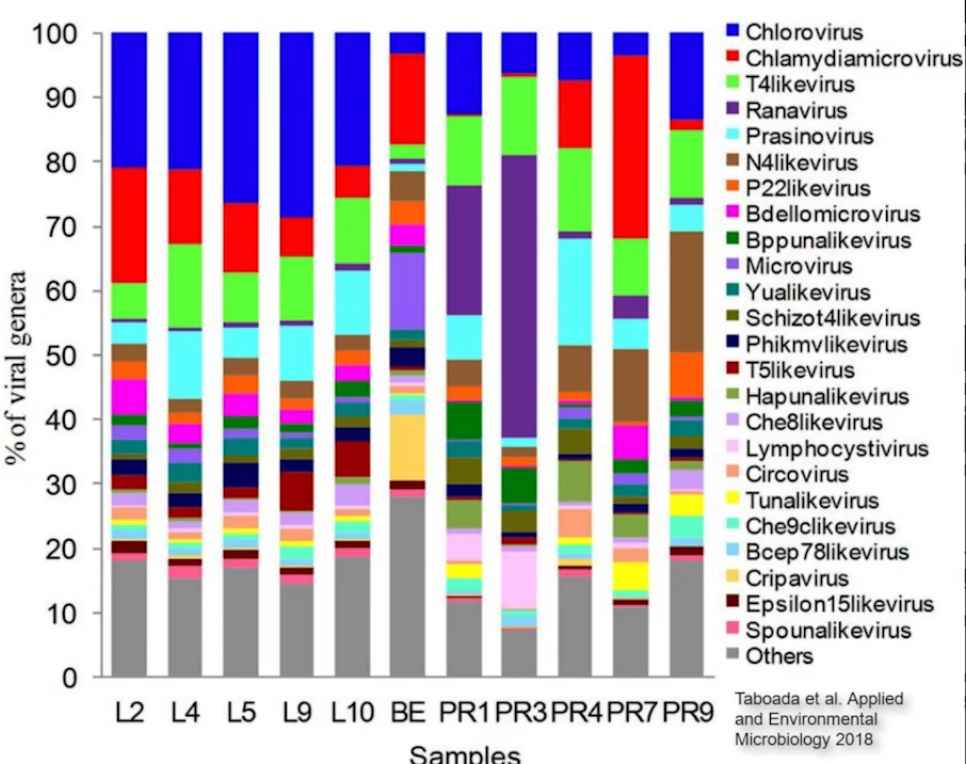
\includegraphics[width=0.8\textwidth]{QuatroCinegasViruses}
\end{figure}

\subsubsection{Nahui Medina: Archaea and extremophiles}
My name is Nahui Medina, and right now I'm a PhD student in Nuevo Le\'on in Monterrey. So, right now I'm doing this amazing project about Archaea and extremophiles. What we do right now is try to isolate every single microorganism that we can, and we do this with amazing people in the lab, trying to create strategies to make these microorganisms live in the lab. This is pretty much interesting because Archaea, you know, in Ancient Greek, is about "ancient," you know. This means that it could help us to know how they lived and try to understand...how life is...what begun... at that moment...it's pretty interesting...

They are so beautiful because they have so many colors - red, pink, and like a... yellowish, some of them. So, it's a pretty amazing project we're doing right now. 
Maybe because it's in a place where the whole ecosystem, and the whole habitat is 
it's not in another place, you know... you cannot find... the species that are in here. So, it's very... interesting because the microorganisms or the prokaryotes are living here. There's just living here and that's it. You cannot find them in another place in the world. So, that's what we're doing and we're so happy to do it.

\subsubsection{Valeria Souza: Posa Azul Two}
\begin{figure}[H]
	\caption{\Gls{gls:poza} Azul Two} 
	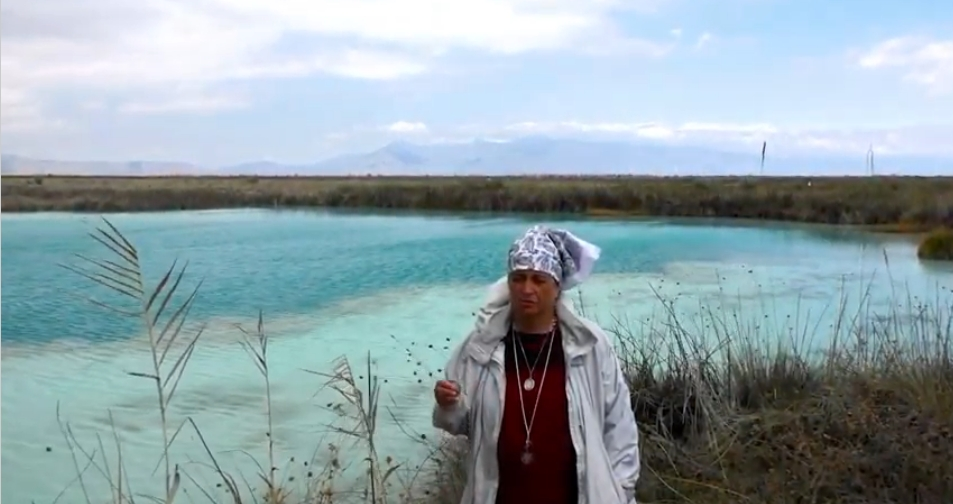
\includegraphics[width=0.9\textwidth]{CuatroCienegas9}
\end{figure}

Here we are in \Gls{gls:poza} Azul Two, that is one of the most beautiful \gls{gls:poza}s in all the valley. What we can see behind us is a very big stromatolite shelf. So, these blue \gls{gls:poza}s take us back to 600 million years ago when the animals changed the chemistry of the ocean and the ocean turned blue --and that's called the Ediacaran Era. So, in Cuatro  Ci\'enegas, we have kind of different timeframes - different moments in geology that got preserved. And, that's really interesting because it's not just a metaphor, it's not just that it looks like the Ediacaran, and when the ocean turned blue, and still the stromatolite shelf were being eaten by the first herbivores -- that was their doom.


But also, it's that this lineage has survived - survived for the longest time. In the Archaean domes that are 50 metres over there--Fugure \ref{fig:PozasAzulesDomes}-- we have evidence that the Archaean - a world of methane and CO2 - is preserved inside domes that are built by bacteria that protect the ancient anaerobic bacteria from the oxygen input--Figure \ref{fig:PozasAzulesDomeInside} while they are doing photosynthesis. This kind of cooperation and construction of the whole niche is pretty unique. We know that stromatolite were world-builders - they made the ocean blue, they transformed every element that came from the start and made life complex. For the fact is that, here in Cuatro  Ci\'enegas, we have a window - a true window - of those lost worlds is really incredible.
\begin{figure}[H]
	\caption{In the Archaean domes that are 50 metres over there} 
	\begin{subfigure}[t]{0.45\textwidth}
		\caption{Archaean Domes}\label{fig:PozasAzulesDomes}
		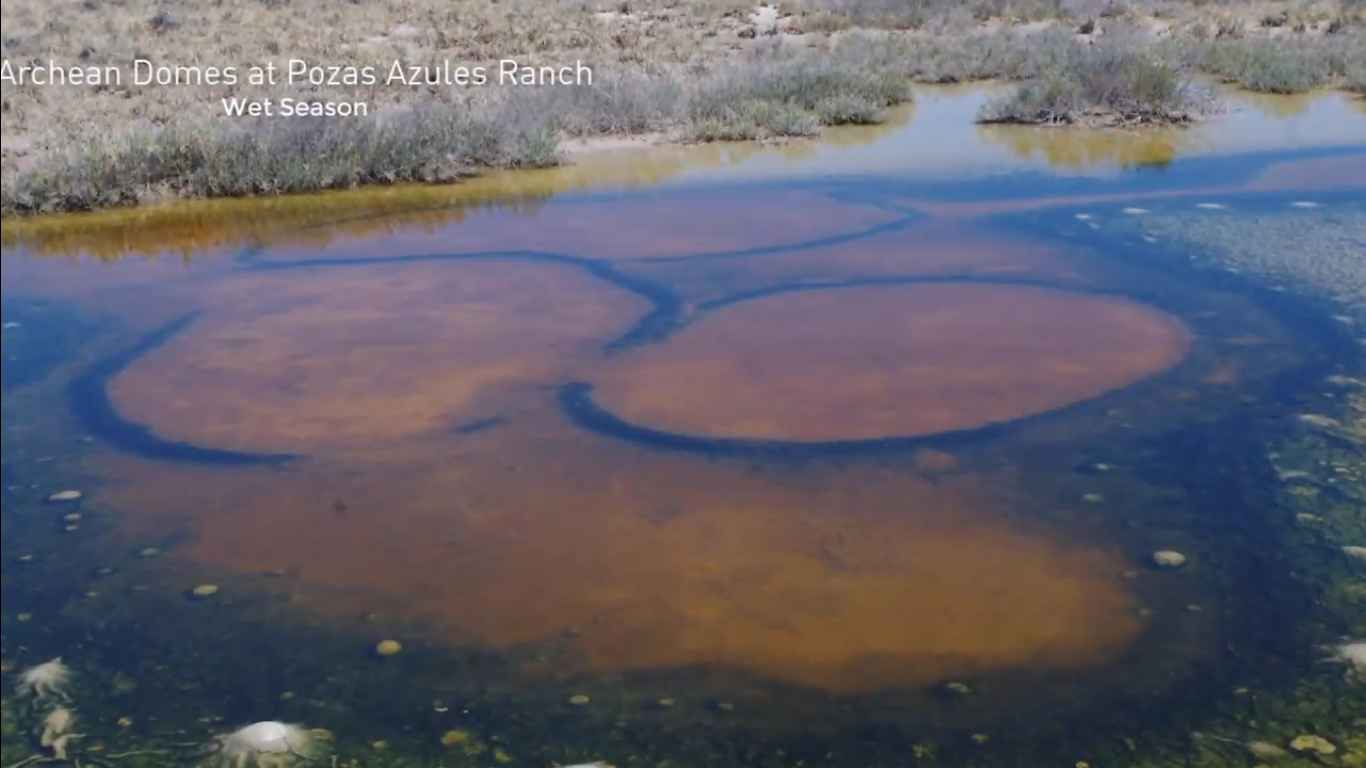
\includegraphics[width=0.9\textwidth]{PozasAzulesDomes}
	\end{subfigure}
	\begin{subfigure}[t]{0.45\textwidth}
		\caption{Inside an Archaean Dome}\label{fig:PozasAzulesDomeInside}
		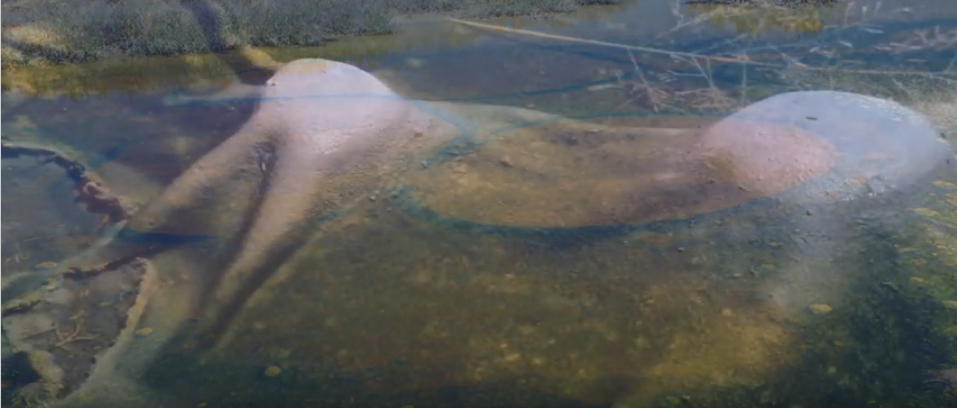
\includegraphics[width=0.9\textwidth]{CuatroCienegas10}
	\end{subfigure}
\end{figure}
Because you walk... meters and you find three billion years... of time. And, you can have lineages that are very, very divergent from the ones we know now, how they assemble their nutrients and how they work. We can cultivate them, we can study them using metagenomics. But, for them to be studied, we need water. And, this water here is precious -it's not just any water. So, water that comes from that mountain that has a magmatic heart, that magmatic heart is responsible for the Jurassic. So, what happened is - humans - we are really silly, and we think we can manage nature. When there's agriculture in the desert... where the water comes comes from -the deep aquifer. And, it is not just any aquifer - it's an aquifer that has stored the conditions of the early sea, and we are losing it.

\begin{figure}[H]
	\caption[The tragedy of Churince where there's no longer water]{Then we have the tragedy of Churince where there's no longer water} 
	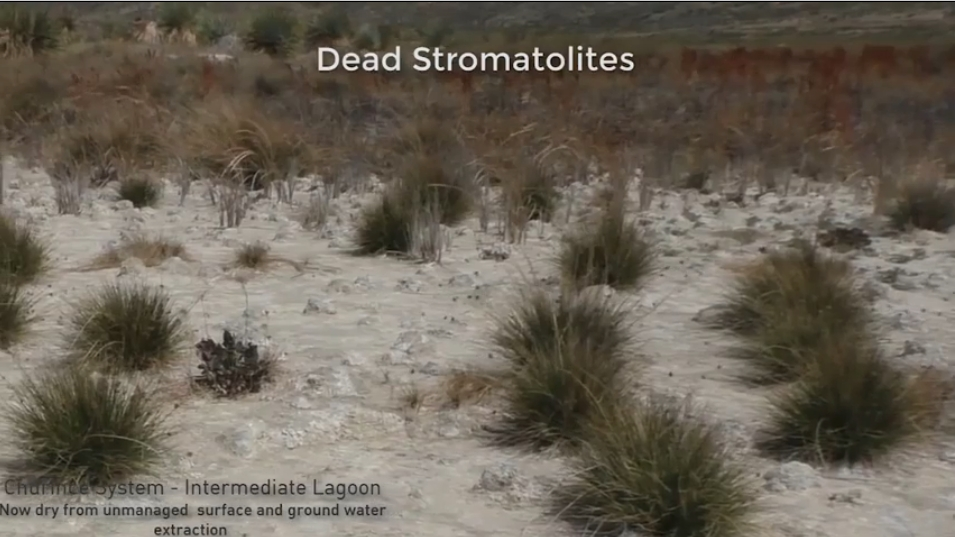
\includegraphics[width=0.9\textwidth]{CuatroCienegas11}
\end{figure}

Then we have the tragedy of Churince where there's no longer water. It only looks like that. And now, it's a field of dead turtles and dead fishes. Maybe there's some hope that we can recover it if we close all the channels that are taking out the water from this ecosystem.

General References:  \cite{gomez2018leptolyngbya,taboada2018geographic}; Phosphates \cite{hao2020cycling,elser2006early}.

\section[Chemistry and The Origins of Life]{Chemistry and The Origins of Life-- Christopher Butch}


We are talking about the origin of life: why are we talking about chemistry? Organic Chemistry is the Chemistry of Life--Figure \ref{fig:Organic Chemistry}: our bodies are made of chemicals, and the processes of the body are chemical reactions. In order to understand where \gls{gls:DNA} and \gls{gls:RNA} come from we need to understand chemistry.


\begin{figure}[H]
	\caption {Organic Chemistry is the Chemistry of Life}\label{fig:Organic Chemistry}
	\begin{subfigure}[b]{0.55\textwidth}
		\includegraphics[width=\textwidth]{OrgChem1}
	\end{subfigure}
	\;
	\begin{subfigure}[b]{0.35\textwidth}
		\includegraphics[width=0.6\textwidth]{OrgChem2}
	\end{subfigure}
\end{figure}

The origin of the scientific field of Origin of Life is the Stanley Miller Experiment\cite{ferus2017formation,miller1953production}--Figure \ref{fig:StanleyMillar}.

\begin{figure}[H]
	\begin{center}
		\caption[The Stanley Miller Experiment]{The origin of the scientific field of Origin of Life is the Stanley Miller Experiment}\label{fig:StanleyMillar}
		\includegraphics[width=0.6\textwidth]{StanleyMillar}
	\end{center}
\end{figure}

What molecules does nature provide? We now have information from molecular clouds in the Universe, from robots on Mars, from meteors, and from deep ocean vents--Figure \ref{fig:NaturalExperiments}. We are trying to understand the chemical inventory from which life was built.
\begin{figure}[H]
	\begin{center}
		\caption{Natural Experiments}\label{fig:NaturalExperiments}
		\includegraphics[width=0.8\textwidth]{NaturalExperiments}
	\end{center}
\end{figure}

It's not enough to know the chemical inventory. There is a problem, which Steve Benner calls the ''Tar problem'': Biomolecules plus heat and time $\rightarrow$ black sludge.\cite{benner2012asphalt}

\begin{itemize}
	\item How do we stop this from happening?
	\item How do we produce useful polymers without making black sludge? 
	\item If we produce black sludge can we somehow turn it into something resembling life?
	\item What molecules can be and are created without life?
	\item How can these molecules be made to react in a life like manner?
	\item How can formation of wasteful byproducts like	tars be prevented?
\end{itemize}


See also \cite{lazcano20031953}

\section[Why Nature Chose Phosphates]{Why Nature Chose Phosphates--Chris Butch}


The role of phosphate in biochemistry and the origins of life.

\subsection{The roles of phosphate in biology}

\begin{itemize}
	\item Structural
	\item Physical
	\item Chemical
\end{itemize}

\subsubsection{Structural role of phosphate}

\begin{itemize}
	\item Nucleic Acid Backbones. \gls{gls:RNA} and \gls{gls:DNA} are linked by phospho-diester bonds--Figure \ref{fig:PhosphoDiesterBond}. The reason is linked to a few properties of phosphorus and its negative charge.
	\begin{itemize}
		\item it repels negatively charged nucleophiles--Figure \ref{fig:PhosphoDiesterBond1}, which would try to break the bond. So the bond is very stable.
		\item it is tunable. If the biochemistry requires the bond to be broken, all it needs to do is position something positive nearby--Figure \ref{fig:PhosphoDiesterBond2}. This is also how nucleic acids are synthesized--Figure \ref{fig:PhosphoDiesterBond3}.
		\item Once the strands have been formed, the charge has an important role in the structure of \gls{gls:RNA} duplexes. It turns out that the phosphates on either strand repel each other, helping to keep the duplex more linear, and the phosphates on each strand repel the other one. This has an important role for keeping the nucleic acid soluble, by keeping them from collapsing in on themselves--Figure \ref{fig:PhosphoDiesterBond3}.
	\end{itemize}
	\item Phospholipid Bilayers. These have a hydrophobic end and a hydrophilic end--Figure \ref{fig:PhosphoLipid1}, which typically has a phosphate and a positively charge portion. Because of this split between hydrophobic and hydrophilic, Phospholipids have a tendency to form two dimensional structures--Figure \ref{fig:PhosphoLipid2}. Zooming out we see the phospholipid layer forming the outer wall of a cell--Figure \ref{fig:PhosphoLipid3}.
\end{itemize}


Phosphates when added to a protein cause a conformational change. This can either activate or inactivate the molecule. A great example is in Protein phosphatase 1 which phosphorylates glycogen synthase causing activation, while also phosphorylating phosphorylase kinase making it inactive\footnote{Comment from Sarah Maurer in Firom}.

\begin{figure}[H]
	\caption{Nucleic Acid Backbones}
	\label{fig:three graphs}
	\begin{subfigure}[b]{0.45\textwidth}
		\centering
		\caption{Phospho Diester Bond}\label{fig:PhosphoDiesterBond} 
		\includegraphics[width=\textwidth]{PhosphoDiesterBond}
	\end{subfigure}
	\begin{subfigure}[b]{0.45\textwidth}
		\centering
		\caption{Repels negatively charged nucleophiles which might break bond, so very stable}\label{fig:PhosphoDiesterBond1} 
		\includegraphics[width=\textwidth]{PhosphoDiesterBond1}
	\end{subfigure}
	\begin{subfigure}[b]{0.45\textwidth}
		\centering
		\caption{Bond is tunable if we need to react}\label{fig:PhosphoDiesterBond2} 
		\includegraphics[width=\textwidth]{PhosphoDiesterBond2}
	\end{subfigure}
	\begin{subfigure}[b]{0.45\textwidth}
		\centering
		\caption{Repulsion keeps  soluble and prevents collapse}\label{fig:PhosphoDiesterBond3} 
		\includegraphics[width=\textwidth]{PhosphoDiesterBond3}
	\end{subfigure}
	
\end{figure}
\begin{figure}[H]
	\caption{Phospholipids}\label{fig:PhosphoLipids}
	\begin{subfigure}[t]{0.3\textwidth}
		\centering
		\caption{Phospholipid Bilayers, showing hydrophobic end and a hydrophilic end.}\label{fig:PhosphoLipid1} 
		\includegraphics[width=\textwidth]{PhosphoLipid1}
	\end{subfigure}\;
	\begin{subfigure}[t]{0.3\textwidth}
		\centering
		\caption{ Because of this split between hydrophobic and hydrophilic, Phospholipids have a tendency to form two dimensional structures}\label{fig:PhosphoLipid2} 
		\includegraphics[width=\textwidth]{PhosphoLipid2}
	\end{subfigure}\;
	\begin{subfigure}[t]{0.3\textwidth}
		\centering
		\caption{Zooming out we see the phospholipid layer forming the outwr wall of a cell.}\label{fig:PhosphoLipid3} 
		\includegraphics[width=\textwidth]{PhosphoLipid3}
	\end{subfigure}
	
\end{figure}

\subsubsection{Physical}

\begin{itemize}
	\item Compartmentalization--Figure \ref{fig:Compartmentalization}. By having this charged barrier, biochemistry can determine what can and cannot go into a cell. An example is the reaction of 2 3Carbon to form a 6Carbon--Figure \ref{fig:CompartmentalizationExample}. Although phosphorus isn't involved--the atoms are at the opposite ends of the two chains--the phosphoralization is preserved, and this is a motif. It keeps the sugars inside the cell.
	\item Signaling Some examples of how phosphates are used in signaling are in the signaling cascades where proteins are phosphorylated or cAMP is generated.
\end{itemize}

\begin{figure}[H]
	\caption{Phosphates allow physical Compartmentalization}\label{fig:Compartmentalization}
	\begin{subfigure}[t]{0.35\textwidth}
		\caption{Charged molecules can be stopped, but not uncharged}
		\includegraphics[width=\textwidth]{Compartmentalization}
	\end{subfigure}\;
	\begin{subfigure}[t]{0.5\textwidth}
		\caption{Example: Glycolosis and Gluconeogenesis }\label{fig:CompartmentalizationExample}
		\includegraphics[width=\textwidth]{CompartmentalizationExample}
	\end{subfigure}
\end{figure}
\subsubsection{Chemical}

\begin{itemize}
	\item Energy--Figure \ref{fig:ATP}. ''On any given day you turn over your body weight equivalent in \gls{gls:ATP}, the principal energy currency of the cell''--\cite{tornroth2008opening}. The reason is the energy of the Triphosphate can be used to transfer phosphate to other molecules--Figure \ref{fig:ATP1}
	\item Activation Once you have tranferred phosphorous, it can be used as leading group to promote a reaction that would not otherwise be favourable--Figure \ref{fig:Synthesis-beta-5-phosphorybosylamine}. 
\end{itemize}

\begin{figure}[H]
	\caption{Adenosine Triphosphate}\label{fig:ATP}
	\includegraphics[width=0.8\textwidth]{ATP}
\end{figure}

\begin{figure}[H]
	\caption[ATP transferring phosphate to other molecules]{The energy of the Triphosphate can be used to transfer phosphate to other molecules. Phosphate can also be used in polymerization.}\label{fig:ATP1}
	\includegraphics[width=0.8\textwidth]{ATP1}
\end{figure}

\begin{figure}[H]
	\caption{Synthesis of $\beta$-5 phosphorybosylamine}\label{fig:Synthesis-beta-5-phosphorybosylamine}
	\includegraphics[width=0.8\textwidth]{Synthesis-beta-5-phosphorybosylamine}
\end{figure}


\subsection{Why wouldn't you use phosphate?}

\subsubsection{Phosphate is quite scarce\cite{keefe1995polyphosphates}}
\begin{itemize}
	\item Insoluble, un-reactive (tied up in minerals that are not available for life)
	\item No polyphosphate minerals
	\item One pyrophosphate mineral
	\item Limited geochemical production of reactive forms
\end{itemize}
\subsubsection{Open Questions--\cite{life2017special}}

\begin{itemize}
	\item How did life begin to use phosphate?
	\item When did life begin to use phosphate?
	\item If not at the very beginning, what came before?\cite{goldford2017remnants}
	\item Where did early phosphate come from?
\end{itemize}

See also \cite{westheimer1987nature,soderberg2019organic}

\section{Why Water? Why Carbon?}

\subsection{Why Water? Why Carbon?}

\begin{itemize}
	\item All life on earth is based on reactions of carbon and water.
	\item Why? What are the options?
\end{itemize}

Figures \ref{fig:abundances1} and \ref{fig:abundances2} show abundances. Figure \ref{fig:minerals} shows elements likely to be locked up in minerals, Figure \ref{fig:volatiles} shows elements that are likely to be in atmosphere or sea. Bonds are important - carbon has 4.

\begin{figure}[H]
	\caption{Abundance of Elements in the Solar System}\label{fig:abundances1} 
	\includegraphics[width=0.9\textwidth]{Abundances}
\end{figure}

\begin{figure}[H]
	\caption{Abundance of Elements in the Earth's Crust}\label{fig:abundances2}  
	\includegraphics[width=0.9\textwidth]{AbundancesEarth}
\end{figure}

\begin{figure}[H]
	\caption[Some elements locked in minerals]{Some elements locked in minerals: they react with oxygen and get locked up.}\label{fig:minerals} 
	\includegraphics[width=0.9\textwidth]{AbundancesMinerals}
\end{figure}

\begin{figure}[H]
	\caption{Some elements volatile}\label{fig:volatiles} 
	\includegraphics[width=0.9\textwidth]{AbundancesGases}
\end{figure}

Abundance isn't the only question. We need to talk about how these elements behave at the electronic level--Figures \ref{fig:Behaviour1} and \ref{fig:Behaviour2}. Carbon is:
\begin{itemize}
	\item the element in Figure \ref{fig:Behaviour2} that is most able to form a diverse set of chemistries;
	\item at the temperatures and pressures on the surface of the earth, is able to adopt a number of different bonding strategies.
\end{itemize}

\begin{figure}[H]
	\caption{how these elements behave at the electronic level}
	\begin{subfigure}[t]{0.5\textwidth}
		\caption{Life is bases on HCON}\label{fig:Behaviour1}
		\includegraphics[width=\textwidth]{Behaviour1}
	\end{subfigure}
	\begin{subfigure}[t]{0.4\textwidth}
		\caption{At the simplest level this is based on the number of electrons that are available.}\label{fig:Behaviour2}
		\includegraphics[width=\textwidth]{Behaviour2}
	\end{subfigure}
	\begin{subfigure}[t]{1.0\textwidth}
	\caption{The role of water in polymerization/de-polymerization.}\label{fig:Polymerization}
	\includegraphics[width=\textwidth]{Polymerization}
\end{subfigure}
\end{figure}

What about water?Polymerization
\begin{itemize}
	\item Hydrogen and oxygen are abundant in the Sun and on Earth;
	\item Water is more stable than $H_2$ and $O_2$;
	\item Water is liquid, which is important for mixing chemical to allow reactivity.
	\item Water is involved in polymerization/de-polymerization--Figure {fig:Polymerization}.
\end{itemize}
	
Water is abundant, stable, and a liquid.

\subsection{What are the other possibilities?}

\subsubsection{What are the other possibilities instead of carbon?}

\begin{itemize}
	\item Silicon
	\begin{itemize}
		\item Can adopt similar structures to carbon
		\item Poor reactivity with many other elements
		\item Reactive with water
	\end{itemize}
	\item Borane
	\begin{itemize}
		\item Diverse Chemistry
		\item Unstable in Oxidizing Environment
		\item Low Cosmic Abundance
	\end{itemize}
	\item Metal Oxides (?)
	\begin{itemize}
		\item 	Less diverse chemistry
		\item Demonstrated biomimetic functions
	\end{itemize}
\end{itemize}

\subsubsection{What are the other possibilities for solvents?}
\begin{itemize}
	\item Ammonia
	\item Urea
	\item Formamide
	\item Alkanes
\end{itemize}

\subsubsection{Open Questions}
\begin{itemize}
	\item What are the surface and atmospheric chemistries of
	exoplanets?
	\item How much of extant biochemistry can be accomplished
	in other solvents?
	\item How much of extant biochemistry can be mimicked with
	other substrates?
\end{itemize}
\section{Macromolecules}

Sarah Maurer

\subsection{Proteins and Lipids}

\subsubsection{Proteins\cite[25.9 Proteins]{brown2009chemistry}}

Proteins are made up of amino acids--Figure \ref{fig:AminoAcids}. Amino acids can be grouped in various ways, based on their side chain--the orange regions in Figure \ref{fig:AminoAcids}. One way to group them is shown in Figure \ref{fig:AminoAcidsGrouped}, where amino acids are grouped by charge. The different groups have different functionality. It is important to have 20 amino acids, so we have a diverse range of functionality in our end product, the protein.

\begin{figure}[H]
	\caption[The full set of 20 amino acids]{The full set of 20 amino acids: blue atoms form protein backbone, orange the sidechain. There are a couple of extra amino acids used for some organisms, but these are the standard set.}\label{fig:AminoAcids} 
	\includegraphics[width=0.8\textwidth]{AminoAcids}
\end{figure}

\begin{figure}[H]
	\caption{Amino acids grouped by charge: non-polar side chains are strongly carbon containing; uncharged polar the side groups contain oxygen, sulphur or nitrogen, with zero nett charge; charged polar the oxygen or nitrogen is negatively or positively charged. }\label{fig:AminoAcidsGrouped} 
	\includegraphics[width=0.8\textwidth]{AminoAcidsGrouped}
\end{figure}
 To get proteins we have to condense two amino acids together--Figure \ref{fig:AminoAcidsCondensed}--by removing a water molecule from the carboxylate and the amine, producing a peptide bond. This can be accomplished by taking an aqueous solution of amino acids and drying them down; this could have happened on early Earth.
\begin{figure}[H]
	\caption{Condensing amino acids by removing $H_2O$. Dehydration.}\label{fig:AminoAcidsCondensed} 
	\includegraphics[width=0.9\textwidth]{AminoAcidsCondensed}
\end{figure}

Proteins have a very specific folded structure--Figure \ref{fig:proteinStructure}--which enables them to recognize their target, a reactant or substrate. The protein and its target fit together like a lock and key: the protein has evolved to match its target.

\begin{figure}[H]
	\caption[Proteins have a very specific folded structure]{Proteins have a very specific folded structure. This example has several $\alpha$-helices and one $\beta$-sheet, represented by an arrow.}\label{fig:proteinStructure}
	\includegraphics[width=0.8\textwidth]{proteinStructure}
\end{figure}

\begin{itemize}
	\item  Need at least several amino acids to have folded stability; most proteins are 50+ amino acids
	\item We would need protein formation to happen many times on early Earth.
	\item Some functional proteins catalyze reactions--either by making or breaking bonds. They are known as "enzymes":
	\begin{itemize}
		\item Lower transition state energy, or;
		\item Orient and concentrate reactants, so they react more quickly than if floating around in solution.
	\end{itemize}
\end{itemize}


\subsubsection{Lipids}

\Glspl{gls:lipid}\cite[14.2 Lipids \& Triglycerides]{brown2009chemistry} are the 2nd type  of biomolecule in this lecture. \glsdesc{gls:lipid}.  \Glspl{gls:lipid} are essential to identifying the individual cells and allow for the cells to undergo Darwinian selection. Lipids form a bilayer--Figure \ref{fig:Lipids}. Water molecules interact with the polar head groups.

\begin{itemize}
	\item \glspl{gls:phospholipid} make up modern cell membranes
	\item other \glspl{gls:amphiphile} can also form membranes
\end{itemize}

\begin{figure}[H]
	\caption[How lipids  allow Darwinian evolution.]{Lipids form hydrophobic membranes that surround cells, and allow Darwinian evolution.}\label{fig:Lipids} 
	\includegraphics[width=0.9\textwidth]{Lipids}
\end{figure}

\begin{itemize}
	\item Most lipids have a glycerol backbone--Figure \ref{fig:LipidTypes}.
	\item You can dehydrate glycerol with a fatty acid to produce glycero fatty acids called glycero esters.
	\item The esters will self assemble into our membranes.
\end{itemize}
\begin{figure}[H]
	\begin{center}
		\caption[Type of lipid depends on head-group]{Type of lipid depends on head-group (blue).}\label{fig:LipidTypes} 
		\includegraphics[width=0.8\textwidth]{LipidTypes}
	\end{center}
\end{figure}
The membrane functionality will depend on the headgroup--Figure \ref{fig:LipidTypes}.

\begin{figure}[H]
	\caption{Chemical Structure of Phospholipids}\label{fig:Phospholipids}
	\includegraphics[width=0.8\textwidth]{Phospholipids}
\end{figure}

\begin{itemize}

	\item some membranes in Achaea, are monolayer not bilayer.
	\item Figure \ref{fig:SimplerLipids} shows some example. Left one has been found in meteorites.
\end{itemize}

Simpler Lipids--Figure \ref{fig:SimplerLipids}?
\begin{itemize}
	\item Single chain amphiphiles with  chemically diverse headgroups
	\item Less stable than phospholipids
\end{itemize}

\begin{figure}[H]
	\caption{Early life would have used simple lipids.}\label{fig:SimplerLipids} 
	\includegraphics[width=0.9\textwidth]{SimplerLipids}
\end{figure}

\subsection{Nucleic Acids \& Sugars}

\subsubsection{Sugars}

Sugars are really important, because they are used for storing energy. They play many role in biological systems:
\begin{itemize}
	\item generating and storing biological energy--Figure \ref{fig:SugarsCycle}.
	\item molecular recognition (as in the immune system)
	\item cellular protection (as in bacterial and plant cell 	walls)
	\item maintaining biological structure (e.g., cellulose).
	\item controlling protein trafficking
	\item cell signaling
	\item cell adhesion
	\item biological lubricants
\end{itemize}

\begin{figure}[H]
	\caption{Sugars: generating biological energy and storing it until we are ready to turn it into \gls{gls:ATP}}.\label{fig:SugarsCycle} 
	\includegraphics[width=0.9\textwidth]{SugarsCycle}
\end{figure}

Sugars have a wide range of structures--Figure \ref{fig:SugarsStructure}.

\begin{figure}[H]
	\caption[Variety of D-\glspl{gls:aldose}]{Variety of D-\glspl{gls:aldose}. When there are 4 carbons there is only one possible structure, but there are 8 structures for 6 carbons. These are known as D-sugars because the second to last carbon has the \emph{OH} on the right hand side. The other carbons have every possible variation to make up the number of variants.}\label{fig:SugarsStructure} 
	\includegraphics[width=0.9\textwidth]{SugarsStructure}
\end{figure}

The double bonded oxygen in the first position makes the sugars in Figure \ref{fig:SugarsStructure} into \glspl{gls:aldehyde}. There is a second type of sugar, \gls{gls:ketose}, that has the doubly bonded carbon in the second position--Figure \ref {fig:ketoses}--i.e. they are \glspl{gls:ketone}. There is less variation among ketoses, but we still have the second to last carbon having an OH on the right hand side, making them D-Sugars.
\begin{figure}[H]
	\caption[Variety of D-ketoses]{Variety of D-ketoses. Because C1 and 2 are not chiral centers there are fewer possible forms for ketoses.}\label{fig:ketoses} 
	\includegraphics[width=0.9\textwidth]{ketoses}
\end{figure}

These sugars are not always linear; they are usually not linear in the body.

\begin{itemize}
	\item Ribose--a 5 carbon sugar from Figure \ref{fig:SugarsStructure}--is usually rolled up into \gls{gls:pyran} (6 member ring) or \gls{gls:furan}(5)
	\item Reactive OH group (green in Figure \ref{fig:SugarTautomers}) is called the ''anomeric Oxygen''; it can be at the bottom ($\alpha$) or top($\beta$). This is where polymerization happens. \gls{gls:RNA} uses $\beta$-furanose form of ribose, which is not the most abundant naturally--Figure \ref{fig:SugarTautomers}--so we need enzymes to make this type.
\end{itemize}

\begin{figure}[H]
	\caption[Sugars can accomplish different functions, depending on shape.]{Sugars are usually not linear: can accomplish different functions, depending on shape.}\label{fig:SugarTautomers} 
	\includegraphics[width=0.9\textwidth]{SugarTautomers}
\end{figure}

Sugars can be made prebiotically from the formose reaction--Figure fig:{SugarsPrebioticSynthesis}. We take small formaldehyde molecules and react them the form larger units. Formaldehyde could be made from carbon dioxode or monoxide and hydrogen

\begin{figure}[H]
	\caption[Prebiotic synthesis of sugars: formose reaction]{Prebiotic synthesis of sugars: formose reaction. As the reaction progresses an insoluble “tar” forms an sugar concentrations decrease!}\label{fig:SugarsPrebioticSynthesis} 
	\includegraphics[width=0.9\textwidth]{SugarsPrebioticSynthesis}
\end{figure}


\subsubsection{Nucleic Acids}

Once we have synthesized our sugars, we start to build nucleic acids. To make a nucleic acid you first need a base--Figure \ref{fig:Nucleobases}. The nitrogen makes these molecules basic.

\begin{figure}[H]
	\caption[The heterocyclic bases are
	derivatives of \gls{gls:purine} and of \gls{gls:pyrimidine}]{The two types of heterocyclic bases are
		derivatives of \gls{gls:purine} and of \gls{gls:pyrimidine}.}\label{fig:Nucleobases} 
	\includegraphics[width=0.9\textwidth]{Nucleobases}
\end{figure}

Nucleic acids can base-pair--Figure \ref{fig:BasePairs} to perform specific recognition.
\begin{figure}[H]
	\caption[A-T  and G-C are the base pairs in the Watson–
		Crick model]{A-T (2 H-bonds) and G-C (3 H-bonds) are the base pairs in the Watson–
		Crick model of \gls{gls:DNA}.}\label{fig:BasePairs} 
	\includegraphics[width=0.9\textwidth]{BasePairs}
\end{figure}

{Prebiotic synthesis is challenging, but not impossible--Figure \ref{fig:PrebioticSynthesis}. We start with methane and ammonia, and there are several pathways to produces the bases.
\begin{figure}[H]
	\caption{Prebiotic synthesis is challenging, but not impossible!}\label{fig:PrebioticSynthesis} 
	\includegraphics[width=0.9\textwidth]{PrebioticSynthesis}
\end{figure}
Once we have the bases we can add them to our Ribose--Figure \ref{fig:NucleotideStructure}.
\begin{itemize}
	\item Ribose and phosphate make up backbone.
	\item Bases on outside, so can basepair.
	\item Notice the loss of oxygen going from \gls{gls:RNA} to \gls{gls:DNA}. The OH is important in forming hydrogen bonds, which allow \gls{gls:RNA} to form complex structures, and allows for functionality. 
	\item The Phosphate is used to polymerize nucleic acids: phosphate, sugar,  phosphate, sugar, ....
\end{itemize}
\begin{figure}[H]
	\caption{Nucleotide Structure.  }\label{fig:NucleotideStructure} 
	\includegraphics[width=0.9\textwidth]{NucleotideStructure}
\end{figure}


\begin{figure}[H]
	\caption{Nucleic Acid Polymers. Bases are added to reactive end of Ribose.}\label{fig:NucleicAcidPolymers} 
	\includegraphics[width=0.9\textwidth]{NucleicAcidPolymers}
\end{figure}

\begin{itemize}
	\item Each monomer is presented as an NTP to be added to the chain.
	\begin{itemize}
		\item Prebiotic way is to dry the chemicals.
		\item In out body we split ATP, which releases energy to drive reaction.
	\end{itemize}
	\item Cleavage of the NTP provides the free energy that makes the reaction
	thermodynamically favorable.
	\item The enzymes catalyzing such reactions are
	called 	\textit{polymerases}.
	\item Mixing all of the biomolecules together in the
	appropriate ratios that living things have, does not
	create life.
	\item \textit{What is missing?}
\end{itemize}

\cite[19.S, Nucleic Acids (Summary)]{brown2009chemistry} 
\cite{xu2020selective,bhowmik2019role}
\section{Chemical Cycles and Chaos}

Chris Kempes

\subsection{Introduction}

What properties and processes are ''easy'' to obtain through physical dynamics alone?
\begin{itemize}
	\item Limit cycle--Figure \ref{fig:LimitCycle};
	\item Chaotic Dynamics--Figure \ref{fig:ChaoticDynamics}.
\end{itemize}

\begin{figure}[H]
	\caption{Processes that are easy to obtain through physical dynamics alone}
	\begin{subfigure}[t]{0.45\textwidth}
		\caption{Limit Cycle}\label{fig:LimitCycle}
		\includegraphics[width=0.8\textwidth]{LimitCycle}
	\end{subfigure}
	\begin{subfigure}[t]{0.45\textwidth}
		\caption{Chaotic Dynamics}\label{fig:ChaoticDynamics}
		\includegraphics[width=\textwidth]{ChaoticDynamics}
	\end{subfigure}
\end{figure}

\subsection{Simulation}

We've been talking about how limit cycles and chaotic dynamics naturally lead to cycling behaviour. The \textit{Brusselator} is an abstract set of chemical reactions that exhibits the behaviour.

\begin{align*}
	A \rightarrow& X\\
	B + X \rightarrow& Y + D\\
	2X + Y \rightarrow& 3X \\
	X \rightarrow& E
\end{align*}

These can be described by differential equations:

\begin{align*}
\dot X =& k_1 A - k_2 B X + k_3 X^2 Y -k_4 X\\
\dot Y =& k_2 B X -k_3 X^2 Y  
\end{align*}

Assuming that we hold concentrations of $A$ and $B$ constant in system. We can non-dimensionalize:
\begin{align*}
\dot x =& a - b x +x^2 y -x\\
\dot y =& bx - x^2 y\text{, which has steady state}\\
x^* =& a\\
y^* =& \frac{b}{a}
\end{align*}

Steady state is unstable for $b>a^2+1$. 

\begin{figure}[H]
	\caption[Brusselator Stability and Phase Plane]{Brusselator Stability. Figures \ref{fig:BrusselatorPhase1} through \ref{fig:BrusselatorPhase3} show the behaviour in the Phase Plane}\label{fig:BrusselatorStability}
	
	\begin{subfigure}[b]{0.3\textwidth}
		\centering
		\caption{ $b\ll a^2+1$--stable}\label{fig:BrusselatorSteadyState1} 
		\includegraphics[width=\textwidth]{BrusselatorSteadyState1}
	\end{subfigure}
	\begin{subfigure}[b]{0.3\textwidth}
		\centering
		\caption{$b<a^2+1$, but close! Transient exhibits oscillations, which ring down to steady state.}\label{fig:BrusselatorSteadyState2} 
		\includegraphics[width=\textwidth]{BrusselatorSteadyState2}
	\end{subfigure}
	\begin{subfigure}[b]{0.3\textwidth}
		\centering
		\caption{$b>a^2+1$}\label{fig:BrusselatorChaos} 
		\includegraphics[width=\textwidth]{BrusselatorChaos}
	\end{subfigure}
	\begin{subfigure}[b]{0.3\textwidth}
		\centering
		\caption{ $b\ll a^2+1$--stable}\label{fig:BrusselatorPhase1} 
		\includegraphics[width=\textwidth]{BrusselatorPhase1}
	\end{subfigure}
	\begin{subfigure}[b]{0.3\textwidth}
		\centering
		\caption{$b<a^2+1$, but close!}\label{fig:BrusselatorPhase2} 
		\includegraphics[width=\textwidth]{BrusselatorPhase2}
	\end{subfigure}
	\begin{subfigure}[b]{0.3\textwidth}
		\centering
		\caption{$b>a^2+1$--Limit Cycle}\label{fig:BrusselatorPhase3} 
		\includegraphics[width=\textwidth]{BrusselatorPhase3}
	\end{subfigure}
\end{figure}

The dynamics is completely deterministic.

See also \cite{ault2003dynamics}.

A classic system for chaos is the Lorentz system. Depending on the parameters the Lorentz system can exhibit stability--Figure \ref{fig:Lorentz}, Limit Cycles, or chaos--Figure \ref{fig:ChaoticDynamics}.

\begin{align*}
	\dot{x} =& \sigma (y-x)\\
	\dot{y} =& x(\rho-z)-y\\
	\dot{z} =& xy-\beta x
\end{align*}

\begin{figure}[H]
	\caption{Stable configuration of Lorentz System}\label{fig:Lorentz}
	\includegraphics[width=0.8\textwidth]{Lorentz}
\end{figure}
% end of text 

Additional references from Office Hours: \cite{maurer2017impact,forsythe2015ester,vincent2019chemical,mehta2018caveats}


% glossary : may need command makeglossaries.exe origins2
\printglossaries

% bibliography goes here
 
\bibliographystyle{unsrt}
\addcontentsline{toc}{section}{Bibliography}
\bibliography{origins,wikipedia}

\end{document}
